\chapter{Setting Up the Input File for CFAST}

\section{Overview}

CFAST is a computer program that uses an input file and generates one or more output files. The first step in performing a calculation is to generate a text input file that provides the program with all of the necessary information to describe the scenario under consideration.  The most important inputs determine the geometry of the compartments in the scenario and the connections between these compartments. Next, the fire, detection, and suppression characteristics of the scenario are defined. Finally, there are a number of parameters that customize the output from the model.  Each line of the file contains a keyword label that identifies the input, followed by a number of numerical or text inputs corresponding to the particular input keyword. A simple input file is shown below. This example is used in the discussion of the output in Chapter 5.

\begin{lstlisting}
VERSN,6,Cable tray fire -- base case
!!
!!Scenario Configuration Keywords
!!
TIMES,1800,-120,10,30
EAMB,293.15,101300,0
TAMB,293.15,101300,0,50
CJET,WALLS
WIND,0,10,0.16
!!
!!Material Properties
!!
MATL,CONCRETE,1.75,1000,2200,0.15,0.94,"Concrete, Normal Weight (6 in)"
MATL,GLASSFB3,0.036,795,105,0.013,0.9,"Glass Fiber, Organic Bonded (1/2 in)"
MATL,METHANE,0.07,1090,930,0.0127,0.04,"Methane, a transparent gas (CH4)"
MATL,HARDWOOD,0.16,1255,720,0.019,0.9,"Wood, Hardwoods (oak, maple) (3/4 in)"
!!
!!Compartment keywords
!!
COMPA,Compartment 1,9.1,5,4.6,0,0,0,GLASSFB3,CONCRETE,CONCRETE
!!
!!Vent keywords
!!
HVENT,1,2,1,1,2.4,0,1,0,0,1,1
!!
!!Fire keywords
!!
GLOBA,10,393.15
!!Wood_Wall
FIRE,1,4.55,2.5,0,1,1,0,0,0,1,Wood_Wall
CHEMI,1,4,0,0,0,0.33,1.81E+07,HARDWOOD
TIME,0,8000
HRR,0,1000000
SOOT,0.02,0.02
CO,0.02,0.02
TRACE,0,0
AREA,0.05,9
HEIGH,0,3
!!
!!Target and detector keywords
!!
TARGET,1,2.2,1.88,2.34,0,0,1,CONCRETE,IMPLICIT,PDE,0.5
\end{lstlisting}

All of the inputs to the model are discussed in this chapter.  Following the discussion that details each input, their engineering units and default values, notes are included that provided additional guidance or frequently addressed problems that may be encountered by the user. These notes take the form of a bulleted list such as:

\begin{itemize}
\item The inputs may be integers (e.g., a simulation time of 1800 s), real numbers (a mass loss rate of 0.0082 kg/s), or text (a floor material of CONCRETE), as appropriate. The input file is a comma-separated ASCII text file and may be edited with a spreadsheet program or any text editor. It is possible to use a word processor but it is important to save the file in ASCII text format and not in a word processing format. Note that some word processors will save punctuation and other characters incorrectly for the simple ASCII text file used by CFAST. It is recommended that the input files be created with the input editor, CEdit, provided as part of the CFAST distribution.  In addition to checking the input data for errors, it includes typical ranges for input values to assist in appropriate use of the model.

\item Numeric format for inputs to CFAST and the input editor CEdit assume a period is used to separate the integer and fractional parts of the number. No separator is used to group digits in the integer part of numbers.

\item Each line of input consists of a label followed by one or more alphanumeric parameters associated with that input label, separated by commas.  The label must always begin in the first space of the line and be in capital letters.  Following the label, the values may start in any column, and all values must be separated by a comma.  Values may contain decimal points if needed or desired.  They are not required.  

\item Inputs are in standard SI units.  The maximum line length is 1024 characters, so all data for each keyword must fit in this number of characters.
\end{itemize}

The installation program creates a shortcut to the input editor on the Windows start menu labeled "CFAST" that points to the input editor.  Once started, the user is presented with a series of tabbed-pages for the various inputs in a CFAST input data file.

\begin{figure}[h!]
\begin{center}

\includegraphics[width=6.5in]{FIGURES/Input_File/Tabs}
\end{center}
\end{figure}

These tabbed-pages organize the inputs for CFAST simulations into several categories as follows.
\begin{itemize}
\item \textbf{Simulation Environment} includes simulation time, specification of model outputs, and ambient conditions. Also included on the page are a constantly updated list of errors, warnings, and messages about the input file specification or model simulation.
\item \textbf{Compartment Geometry} defines the size, construction characteristics, and position of the compartments in a simulation.
\item \textbf{Wall Vents, Ceiling/Floor Vents, and Mechanical Flow Vents} allows the user to connect compartments with doors and windows, ceiling and floor vents, or forced air ventilation systems.
\item \textbf{Fires} include user specification of the initial fire source and any additional burning objects in one or more of the compartments of the simulation.
\item \textbf{Detection / Suppression}defines any heat alarms and sprinklers in the compartments of the simulation.
\item \textbf{Targets} provide the ability calculate the temperature and net heat flux to objects placed and oriented arbitrarily in the structure.
\item \textbf{Surface Connections} allows for more detailed description of the connections between compartments in the simulation to better simulate the transfer of heat from compartment to compartment in the simulation.
\end{itemize}

Each of these tabbed-pages is described in more detail below. In addition, a series of menus allow the user to open and save files; run the simulation, or access help and program information.

\newpage
\section{Simulation Environment}

The Simulation Environment page defines the initial conditions and simulation time for the CFAST input file. 

\begin{figure}[h!]
\begin{center}
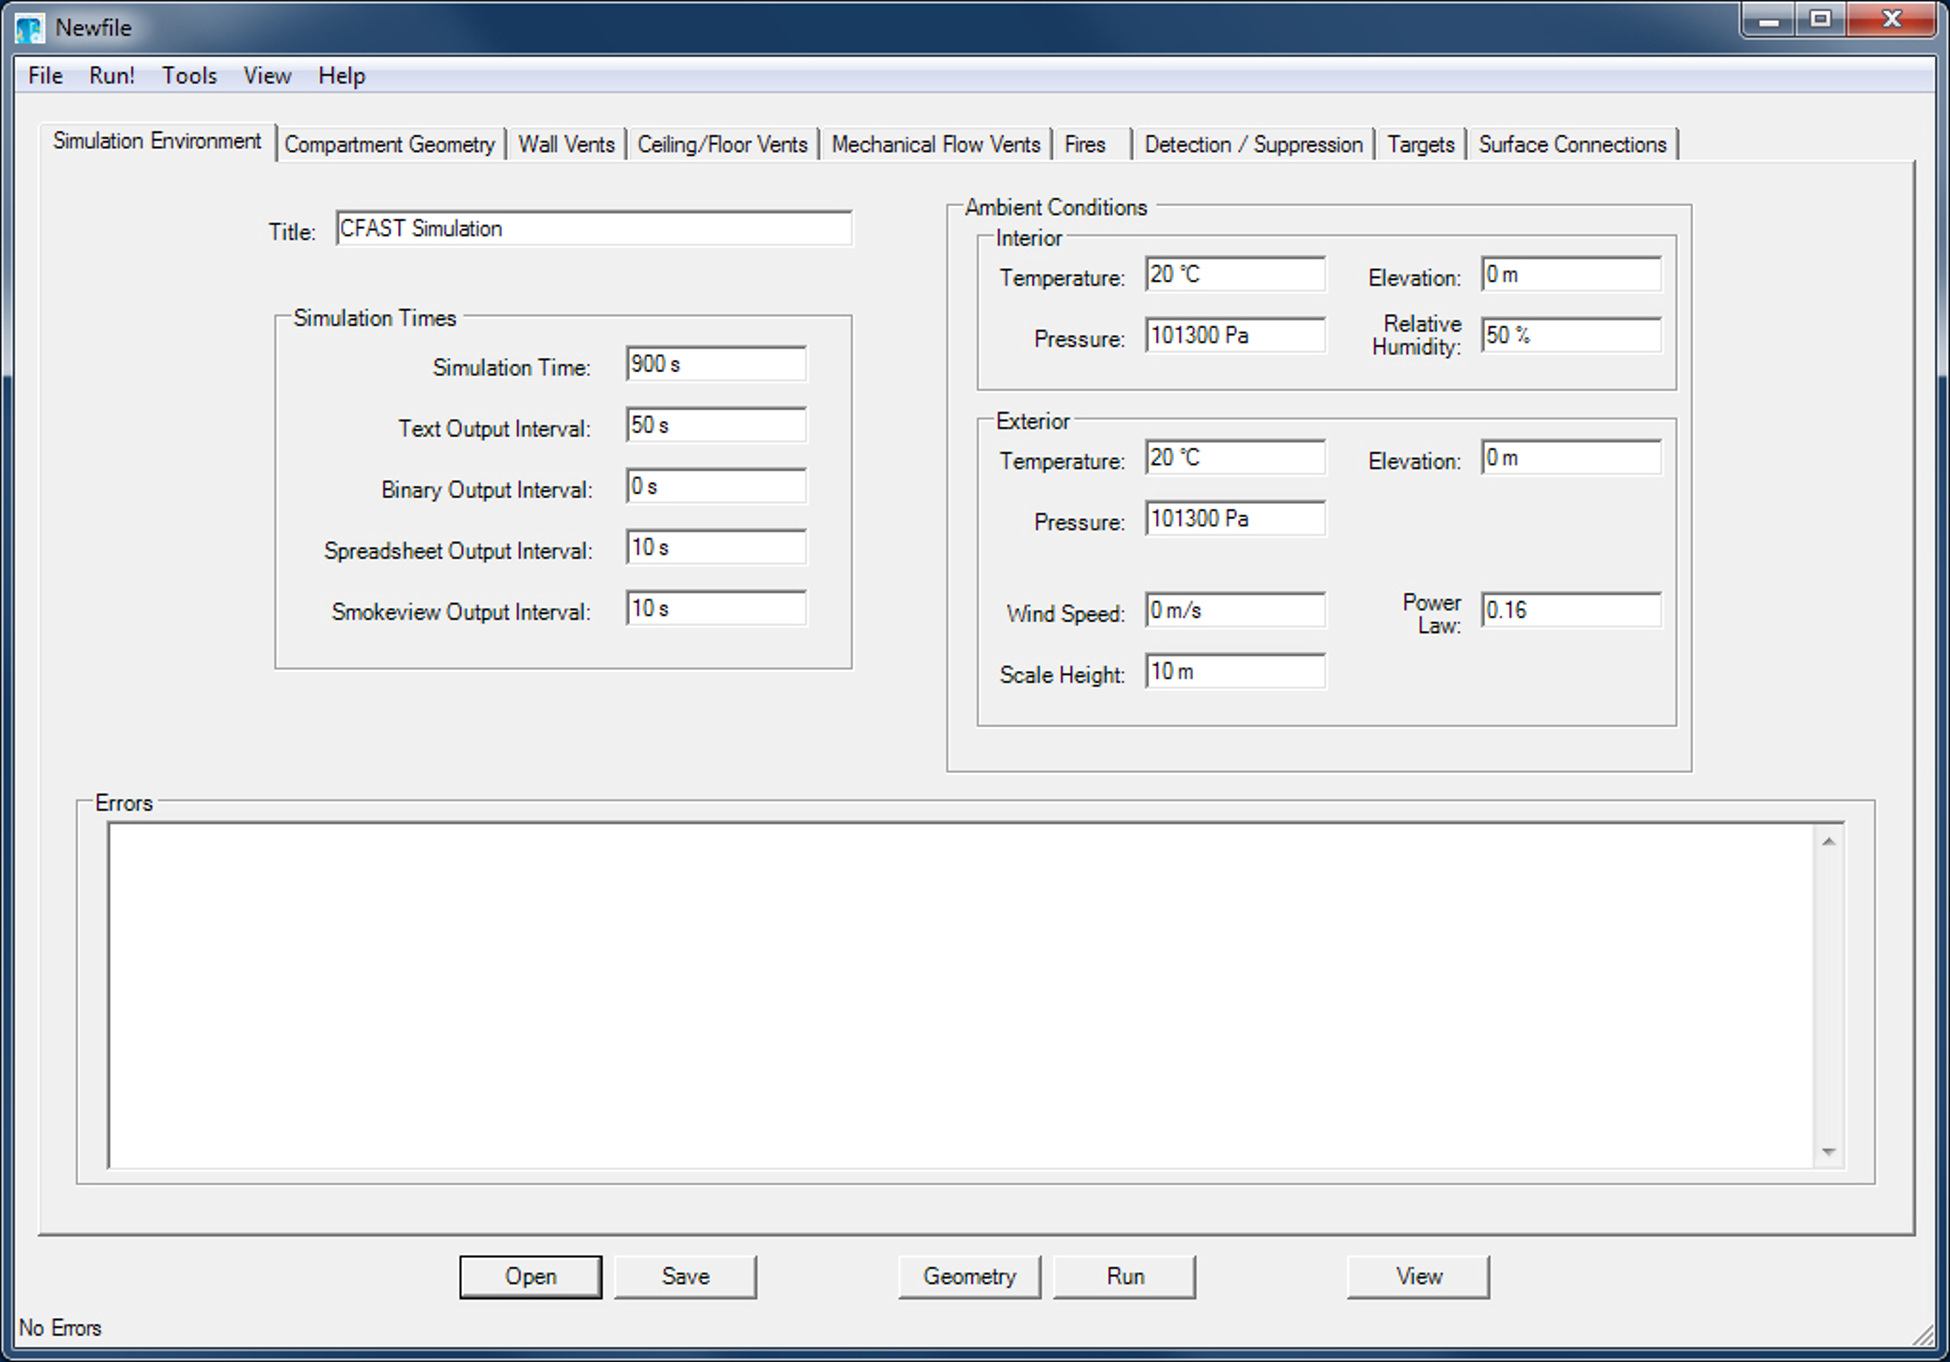
\includegraphics[width=6.5in]{FIGURES/Input_File/Environment_Tab}
\end{center}
\end{figure}

\subsection{Naming the Calculation, the Title Input}

The first thing to do when setting up an input file is to give the simulation a title.  The first line in the CFAST input data file must be the CFAST version identification along with an optional short title for the simulation.  This is a required input.  The title command is the line that CFAST keys on to determine whether it has a correct data file.

\begin{lstlisting}
VERSN,6,CFAST Simulation
\end{lstlisting}

\clearpage

\begin{figure}[h!]
\begin{center}

\includegraphics[width=3.458in]{FIGURES/Input_File/Title}
\end{center}
\end{figure}

\textbf{Title:} The title is optional and may consist of letters, numbers, and/or symbols and may be up to 50 characters. It permits the user to label each run.

\subsection{Setting Time Limits and Output Options}

A TIMES line specifies the length of time over which the simulation takes place and how often output will be generated. This is a required input. There are one to four entries in this line.

\begin{lstlisting}
TIMES,900,50,10,10
\end{lstlisting}

\begin{figure}[h!]
\begin{center}
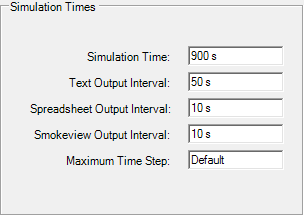
\includegraphics[width=3.167in]{FIGURES/Input_File/Simulation_Times}
\end{center}
\end{figure}

\begin{itemize}
\item \textbf{Simulation Time} (default units: s, default value, 900 s): The length of time over which the simulation takes place.  This is a required input which should be entered even if all other fields are not included. The maximum value for this input is 86400 s (1 day).

\item \textbf{Text Output Interval} (default units: s, default value, 50 s): The print interval is the time interval between each printing of the output values.  If omitted or less than or equal to zero, no output values will occur.

\item \textbf{Spreadsheet Output Interval} (default units: s, default value, 10 s): CFAST can output a subset of the results of the model simulation in a comma-delimited alphanumeric format which can be read by most spreadsheet software. This is designed to be imported into a spreadsheet for further analysis or graphing of the results of the simulation.  This input defines the time interval between outputs of the model results in a spreadsheet-compatible format. A value greater than zero must be used if the spreadsheet file is to be used.

\item \textbf{Smokeview Output Interval} (default units: s, default value: 10 s): CFAST can output a subset of the results in a format compatible with the visualization program smokeview. This input defines the time interval between outputs of the model results in a smokeview-compatible format.  A value greater than zero must be used if the spreadsheet output is desired.
\end{itemize}

In addition to the input data file created specifically for a CFAST simulation, there are a number files that CFAST uses to define default values and other input information, and to output the results of the simulation for later analysis.  They include 1) a thermal properties file, 2) files of predefined fire objects, and 4) a spreadsheet-compatible output file.

The thermal properties file contains material properties for compartment surfaces, target objects that may be placed in compartments in the simulation to monitor surface temperature and heat flux to the objects, and fire objects, in addition to the main fire in the simulation that may ignite based on their surface temperature or incident flux onto the surface of the object. The predefined fire objects files contain definitions for a number of reference fires from the literature or developed by the user that may be included in a simulation. The thermal properties and fire objects files may be modified by the user.  Details of the files are included in the appendices.  There are default files included in the CFAST distribution.

\subsection{Ambient Conditions}

Ambient conditions define the environment at which the scenario begins. This allows the user to specify the temperature, pressure, and station elevation of the ambient atmosphere, as well as the absolute wind pressure to which the structure is subjected.  Pressure interior to a structure is calculated simply as a lapse rate (related to the height above sea level) based on the NOAA/NASA tables \cite{GPO:Atmosphere}.  This modification is applied to the vents which connect to the exterior ambient.  The calculated pressure change is modified by the wind coefficient for each vent.  This coefficient, which can vary from -1.0 to +1.0, nominally from -0.8 to +0.8, determines whether the vent is facing away from or into the wind.  The pressure change is multiplied by the vent wind coefficient and added to the external ambient for each vent which is connected to the outside. There is an ambient for the interior and for the exterior of the structure.  Three keywords define the ambient conditions: TAMB for the interior of the structure, EAMB for the exterior of the structure is EAMB, and WIND for the wind information.

\begin{lstlisting}
EAMB,293.15,101300,0
TAMB,293.15,101300,0,50
WIND,0,10,0.16
\end{lstlisting}

\begin{figure}[h!]
\begin{center}
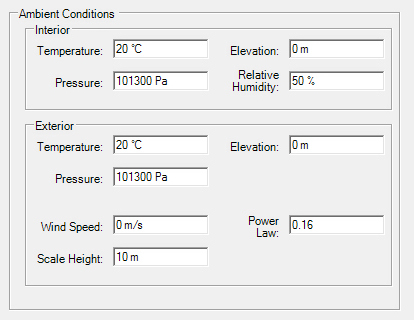
\includegraphics[width=4.313in]{FIGURES/Input_File/Ambient_Conditions}
\end{center}
\end{figure}

\textbf{Ambient Temperature} (default units: \degc~C, default value: 20 \degc~C): Initial ambient temperature inside (for TAMB) or outside (For EAMB) the structure at the station elevation.

\textbf{Ambient Pressure} (default units: Pa, default value: 101300 Pa): Initial values for ambient atmospheric pressure inside (for TAMB) and outside (for EAMB) the structure at the station elevation. Default value is standard atmospheric pressure at sea level (0 m elevation) of 101.3 kPa. Input units are in Pa. These values define standard conditions as defined in Standard Atmosphere as noted in the Handbook of Chemistry and Physics  . There is a set of numerical approximations in the CFAST code which duplicate the pressure/temperature/altitude relationships in the handbook.

\textbf{Elevation} (defaults units: m, default value: 0 m): The height where the ambient pressure and temperature were specified.  This is the reference datum for calculating the density of the atmosphere as well as the temperature and pressure inside and outside of the structure as a function of height.  

\textbf{Relative Humidity} (default units \% RH, default value: 50 \%): The initial relative humidity in the system, only specified for the interior with the TAMB command.  This is converted to kilograms of water per cubic meter.

The wind speed, scale height, and power law are used to calculate the wind coefficient for each vent connected to the outside.  The wind velocity is specified at some reference height.  The power law then provides a lapse rate for the wind speed.  An assumption is that the wind speed is zero at the surface.  The formula used to calculate the wind speed at the height of any vent is show below.  The wind is applied to each external opening as a change in pressure outside of the vent.

\textbf{Wind Speed} (default units: m/s, default value 0 m/s): Wind speed at the reference elevation.

\textbf{Scale Height} (default units: m, default value: 0 m)): Reference height at which the reference wind speed is measured.

\textbf{Power Law Coefficient} (default units: dimensionless, default value 0.16): The power law used to calculate the wind speed as a function of height. Default value is 0.16. Using the notation that $V_W$, is the wind speed at the reference height $H_W$, and $P_W$ is the power law, the exterior pressure is modified by  $\delta P = {C_W}{V^2}$ and $V = {V_W}{\left( {\frac{{{H_i}}}{{{H_W}}}} \right)^{{P_W}}}$ where $H_i$ is the position of the vent \cite{CFAST_Tech_Guide_6}.

\begin{itemize}
\item In order to see the effect of wind, the corresponding parameter for the ventilation keyword must be specified. The default for the wind vector is 0, which turns off wind effects. Please see the HVENT command, below.

\item The choice for station elevation, temperature and pressure must be consistent.  Outside of that limitation, the choice is arbitrary.  It is often convenient to choose the base of a structure to be at zero height and then reference the height of the structure with respect to that height.  The temperature and pressure must then be measured at that position.  Another possible choice would be the pressure and temperature at sea level, with the structure elevations then given with respect to mean sea level.  This is also acceptable, but somewhat more tedious in specifying the construction of a structure.  Either of these choices works though, so long as they are consistent. Usually, the station elevation is set to zero and the pressure to ambient. The effect of changing these values is small for small changes. There will be an effect for places at altitude such as Denver, Colorado, but even there the effect is not pronounced. Note that the equations implemented in the model are not designed to handle negative elevations and altitudes. It is suggested that the defaults be used.

\item These three parameters are optional. If they are not included in the input file, default values are used.
\end{itemize}

\newpage
\section{Compartment Geometry}

The Compartment Geometry page defines the size, position, materials of construction, and flow characteristics for the compartments in the simulation. Initially, only the simulation environment page and the �Add� button on the compartment geometry page is enabled; all other pages are not available to the user for detailed inputs until a compartment has been added to the simulation.  

\begin{figure}[h!]
\begin{center}
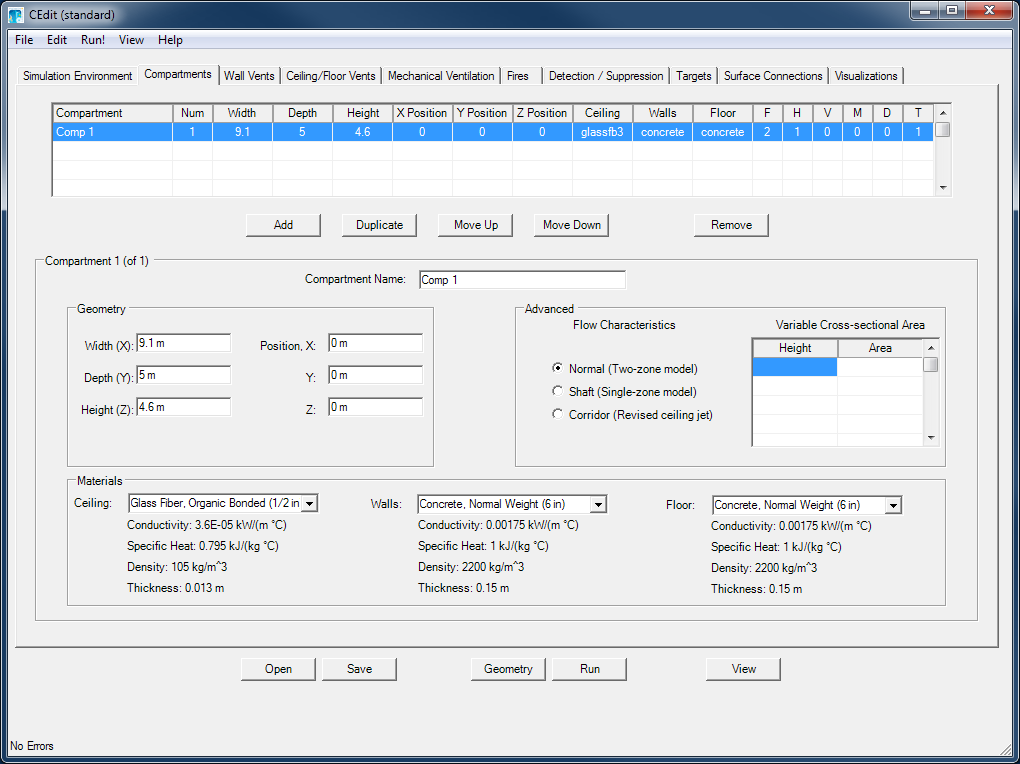
\includegraphics[width=6.5in]{FIGURES/Input_File/Compartment_Geometry_Tab}
\end{center}
\end{figure}

Most of the tabbed pages in the program are of similar design, with a summary of the defined items in table form at the top of the page, a series of buttons to add, remove, or modify the item highlighted in the summary table, and a number of individual inputs below which details all of the inputs for the item selected in the summary table. The buttons included on the compartment geometry page are as follows: \\

\begin{wrapfigure}{l}{0pt}
  
\includegraphics[width=0.781in]{FIGURES/Input_File/Add_Button}
\end{wrapfigure}

Use the Add button to create a new compartment with default values for all entries. \\~ \\

\begin{wrapfigure}{l}{0pt}
  
\includegraphics[width=0.781in]{FIGURES/Input_File/Duplicate_Button}
\end{wrapfigure}

Use the Duplicate button to create a copy of the compartment currently selected in the summary table at the top of the page. The new compartment is added to the end of the list with the named changed to indicate it is a copy of the selected item. \\

\begin{wrapfigure}{l}{0pt}
  
\includegraphics[width=0.781in]{FIGURES/Input_File/Move_Up_Button}
\end{wrapfigure}

Use the Move Up and Move Down buttons to change the order of the list of compartments in the summary table. This simply changes the automatically assigned compartment numbers for the compartments. Compartments can be ordered as desired.

\begin{wrapfigure}{l}{0pt}
  
\includegraphics[width=0.781in]{FIGURES/Input_File/Remove_Button}
\end{wrapfigure}

Use the Remove button to delete the selected compartment from the list of compartments in the summary table.  Other compartments are renumbered once the compartment is deleted.

\subsection{Defining the Compartment}

In order to model a fire scenario, the size and elevation of each compartment in the structure must be specified. For a compartment, the width, depth, compartment height and height of the floor of the compartment provide this specification. The maximum number of compartments for version 6 is thirty. The usual assumption is that compartments are rectangular parallelepipeds. However, the CFAST model can accommodate odd shapes as equivalent floor area parallelepipeds or with a cross-sectional area that varies with height.

At least one compartment must be specified in the input file.  There are no defaults for compartment size. There are defaults for absolute positioning (0,0,0). The fully mixed (single zone) and corridor models are turned off by default.

\begin{wrapfigure}{r}{0pt}
  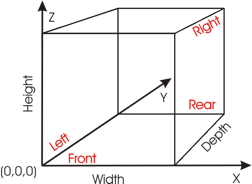
\includegraphics[width=2.0in]{FIGURES/Input_File/CFAST_Coordinates}
\end{wrapfigure}

Compartments in CFAST are most typically defined by a width, depth, and height.  If desired, compartments can be prescribed by the cross-sectional area of the compartment as a function of height from floor to ceiling for other shapes. The absolute position of the compartment with respect to a single structure reference point can be defined to ease visualization or to allow exact placement of vents and surfaces relative to other compartments in a detailed calculation. This specification is important for utilizing the corridor flow algorithm with the HALL command and for positioning the compartments for visualization in SMOKEVIEW. 

The relevant CFAST keywords are COMPA to define the compartment size and materials, HALL or ONEZ to define flow characteristics in the compartment, and ROOMA / ROOMH to define a variable cross-sectional area for the compartment. The COMPA command is required for each compartment as a basic definition for the compartment, even if there are subsequent modifications by the HALL, ONEZ, ROOMA, or ROOMH keywords which follow.  Details of the CFAST keywords are included in Appendix A.

\begin{lstlisting}
COMPA,Compartment 1,9.1,5,4.6,0,0,0,GLASSFB3,CONCRETE,CONCRETE
\end{lstlisting}

\begin{figure}[h!]
\begin{center}

\includegraphics[width=4.0in]{FIGURES/Input_File/Compartment_Name}
\end{center}
\end{figure}

\textbf{Compartment Name:} Compartments are identified by a unique alphanumeric name.  This may be a simple as a single character or number, or a description of the compartment.

\begin{figure}[h!]
\begin{center}
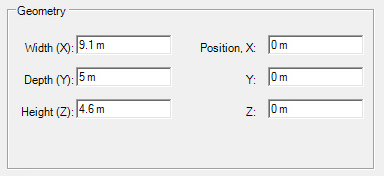
\includegraphics[width=3.552in]{FIGURES/Input_File/Compartment_Size}
\end{center}
\end{figure}

\textbf{Width:} specifies the width of the compartment as measured on the X axis from the origin (0,0,0) of the compartment.  

\textbf{Depth:} specifies the depth of the compartment as measured on the Y axis from the origin (0,0,0) of the compartment.  

\textbf{Height:} specifies the height of the compartment as measured on the Z axis from the origin (0,0,0) of the compartment.  

\begin{wrapfigure}{r}{0pt}
  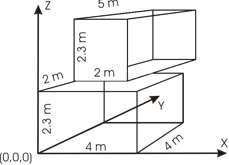
\includegraphics[width=2.0in]{FIGURES/Input_File/CFAST_Absolute_Positioning}
\end{wrapfigure}

\textbf{Absolute Width Position:} specifies the absolute x coordinate of the lower, left, front corner of the room.

\textbf{Absolute Depth Position:} specifies the absolute y coordinate of the lower, left, front corner of the room.

\textbf{Absolute Floor Height:} specifies the height of the floor of each compartment with respect to station elevation specified by the internal ambient conditions reference height parameter.  The reference point must be the same for all elevations in the input data.  For example, the two rooms in the sample to the right would be located at (0,0,0) and (0,2,2.3).

\subsection{Thermal Properties of Bounding Surfaces}

To calculate heat loss through the ceiling, walls, and floor of a compartment, the properties of the bounding surfaces must be known. This includes the thermophysical properties of the surfaces and the arrangement of adjacent compartments if calculation of inter-compartment heat transfer is to be calculated.

The thermophysical properties of the surfaces which define compartments are described by specifying the thermal conductivity, specific heat, emissivity, density, and thickness of the enclosing surfaces for each material and then assigning the material to the ceiling, walls, and floor of a compartment.  Currently, thermal properties for materials are read from the CFAST input file with a thermal database file of common materials included in the CFAST distribution.  The thermophysical properties are specified at one condition of temperature, humidity, etc.  In CFAST version 6, there can only a single layer per boundary (previous versions allowed up to three). 

\begin{lstlisting}
COMPA,Compartment 1,9.1,5,4.6,0,0,0,GLASSFB3,CONCRETE,CONCRETE
\end{lstlisting}

\begin{figure}[h!]
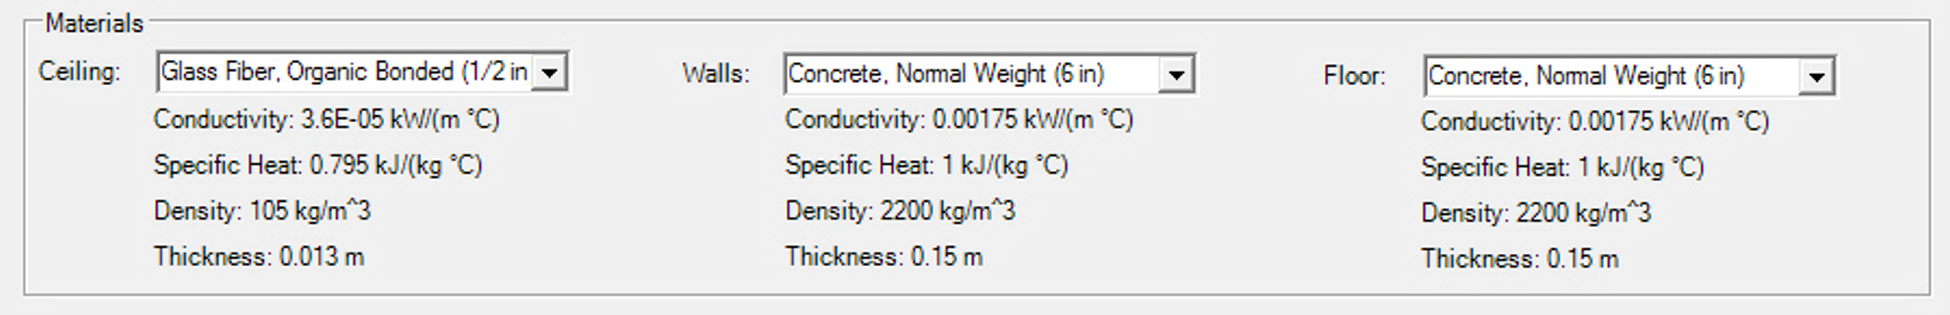
\includegraphics[width=6.5in]{FIGURES/Input_File/Compartment_Materials}
\end{figure}

The bounding surfaces are the ceilings, walls and floors that define a compartment. These are referred to as thermophysical boundaries, since each participates in conduction and radiation as well as defining the compartments, unless these phenomena are explicitly turned off. 

\textbf{Ceiling Material} (default value: Gypsum Board): material name from the thermal properties data file used for the ceiling surface of the compartment. 

\textbf{Wall Material} (default value: Gypsum Board): material name from the thermal properties data file used for the wall surfaces of the compartment.

\textbf{Floor Material} (default value: Off): material name from the thermal properties data file used for the floor surface of the compartment.

\begin{itemize}
\item If the thermophysical properties of the enclosing surfaces are not included, CFAST will treat them as adiabatic (no heat transfer).

\item If a name is used which is not in the database, the model should stop with an error message. The keyword in the data file simply gives a name (such as CONCRETE) which refers to the properties for that material in the thermal data file (see section 4.2.3 and Appendix A for details on the thermophysical database).

\item Since most of the heat conduction is through the ceiling, and since the conduction calculation takes a significant fraction of the computation time, it is recommended that initial calculations be made using the ceiling only.  Adding the walls generally has a small effect on the results, and the floor contribution is usually negligible.  Clearly, there are cases where the above generalization does not hold, but it may prove to be a useful screening technique. A caveat in including floor properties is that the set of equations describing heat transfer becomes difficult to solve once the thermal wave from the compartments reaches the unexposed side of a floor. The back surfaces of compartments are assumed to be exposed to ambient conditions unless specifically specified (see the section on Surface Connections) to specify heat transfer connections between compartments).
\end{itemize}

\newpage
\section{Compartment Connections}

Flow through vents can be natural flow through doors, windows, or openings in ceilings and floors; or forced flow in a mechanical ventilation system.  Natural flow comes in two varieties.  The first is referred to as horizontal flow.  It is the flow which is normally thought of in discussing fires.  It encompasses flow through doors, windows and so on.  The other is vertical flow and can occur if there is a hole in the ceiling or floor of a compartment.  This latter phenomena is useful in some scenarios such as in a ship where openings in floors and ceilings through scuttles are common and in buildings with manual or automatic heat and smoke venting.

Flow through normal vents is governed by the pressure difference across a vent.  There are two situations which give rise to flow through vents.  The first is flow of air or smoke driven from a compartment by buoyancy.  The second type of flow is due to expansion which is particularly important when conditions in the fire environment are changing rapidly.  Rather than depending entirely on density differences between the two gases, the flow is forced by volumetric expansion.

In addition to natural flow, forced flow from mechanical ventilation can affect a fire as well. More important than affecting the fire, however, is the dispersal of the smoke and toxic gases from the fire to adjacent spaces, if ventilation continues to operate after a fire starts.

Atmospheric pressure is about 100 000 Pa. Fires produce pressure changes from 1 Pa to 1000 Pa and mechanical ventilation systems typically involve pressure differentials of about 1 Pa to 100 Pa.  In order to address pressure-induced flow, pressure differences of about 0.1 Pa out of 100 000 Pa for the overall problem or $10^{-4}$ Pa for adjacent compartments must be tracked.

The keywords which describe the various flow regimes are:

\begin{itemize}
\item Windows and doors (horizontal flow through vertical vents): HVENT, specifies vent which connect compartments horizontally
\item Holes in a ceiling/floor (vertical flow through horizontal vents: VVENT, specifies a vent which connects compartments vertically
\item HVAC specification: MVENT specifies a vent which connects compartments with a forced flow
\end{itemize}

For all three types of vents the size of the vent opening (expressed as a fraction of the original opening) may be changed:

\begin{itemize}
\item EVENT change the opening fraction of the specified vent at a chosen time.
\item RAMP change the opening fraction as a function of time by specifying a series of time and fraction pairs
\end{itemize}

Each of these commands is discussed in the sections that follow.

\subsection{Defining Natural Flow Connections Through Doors and Windows}

Horizontal flow connections may include doors between compartments or to the outdoors as well as windows in the compartments.  These specifications do not necessarily correspond to physically connecting the walls between specified compartments.  Rather, lack of an opening simply prevents flow between the compartments.  Horizontal flow connections may also be used to account for leakage between compartments or to the outdoors. 

Horizontal connections can only be created between compartments that physically overlap in elevation at some point. These may include doors between compartments or windows in the compartments (between compartments or to the outdoors).  Openings to the outside are included as openings to a compartment with a number one greater than the number of compartments described in the geometry section.  The relevant CFAST keyword is HVENT.  Details of the CFAST keywords are included in the appendix. It is possible to define a total of 25 horizontal flow connections between any pair of compartments. A number from 1 to 25 uniquely identifies the connection. This number is automatically assigned by the input editor based on the order they appear in the summary table on the horizontal flow vents page.

\begin{figure}[h!]
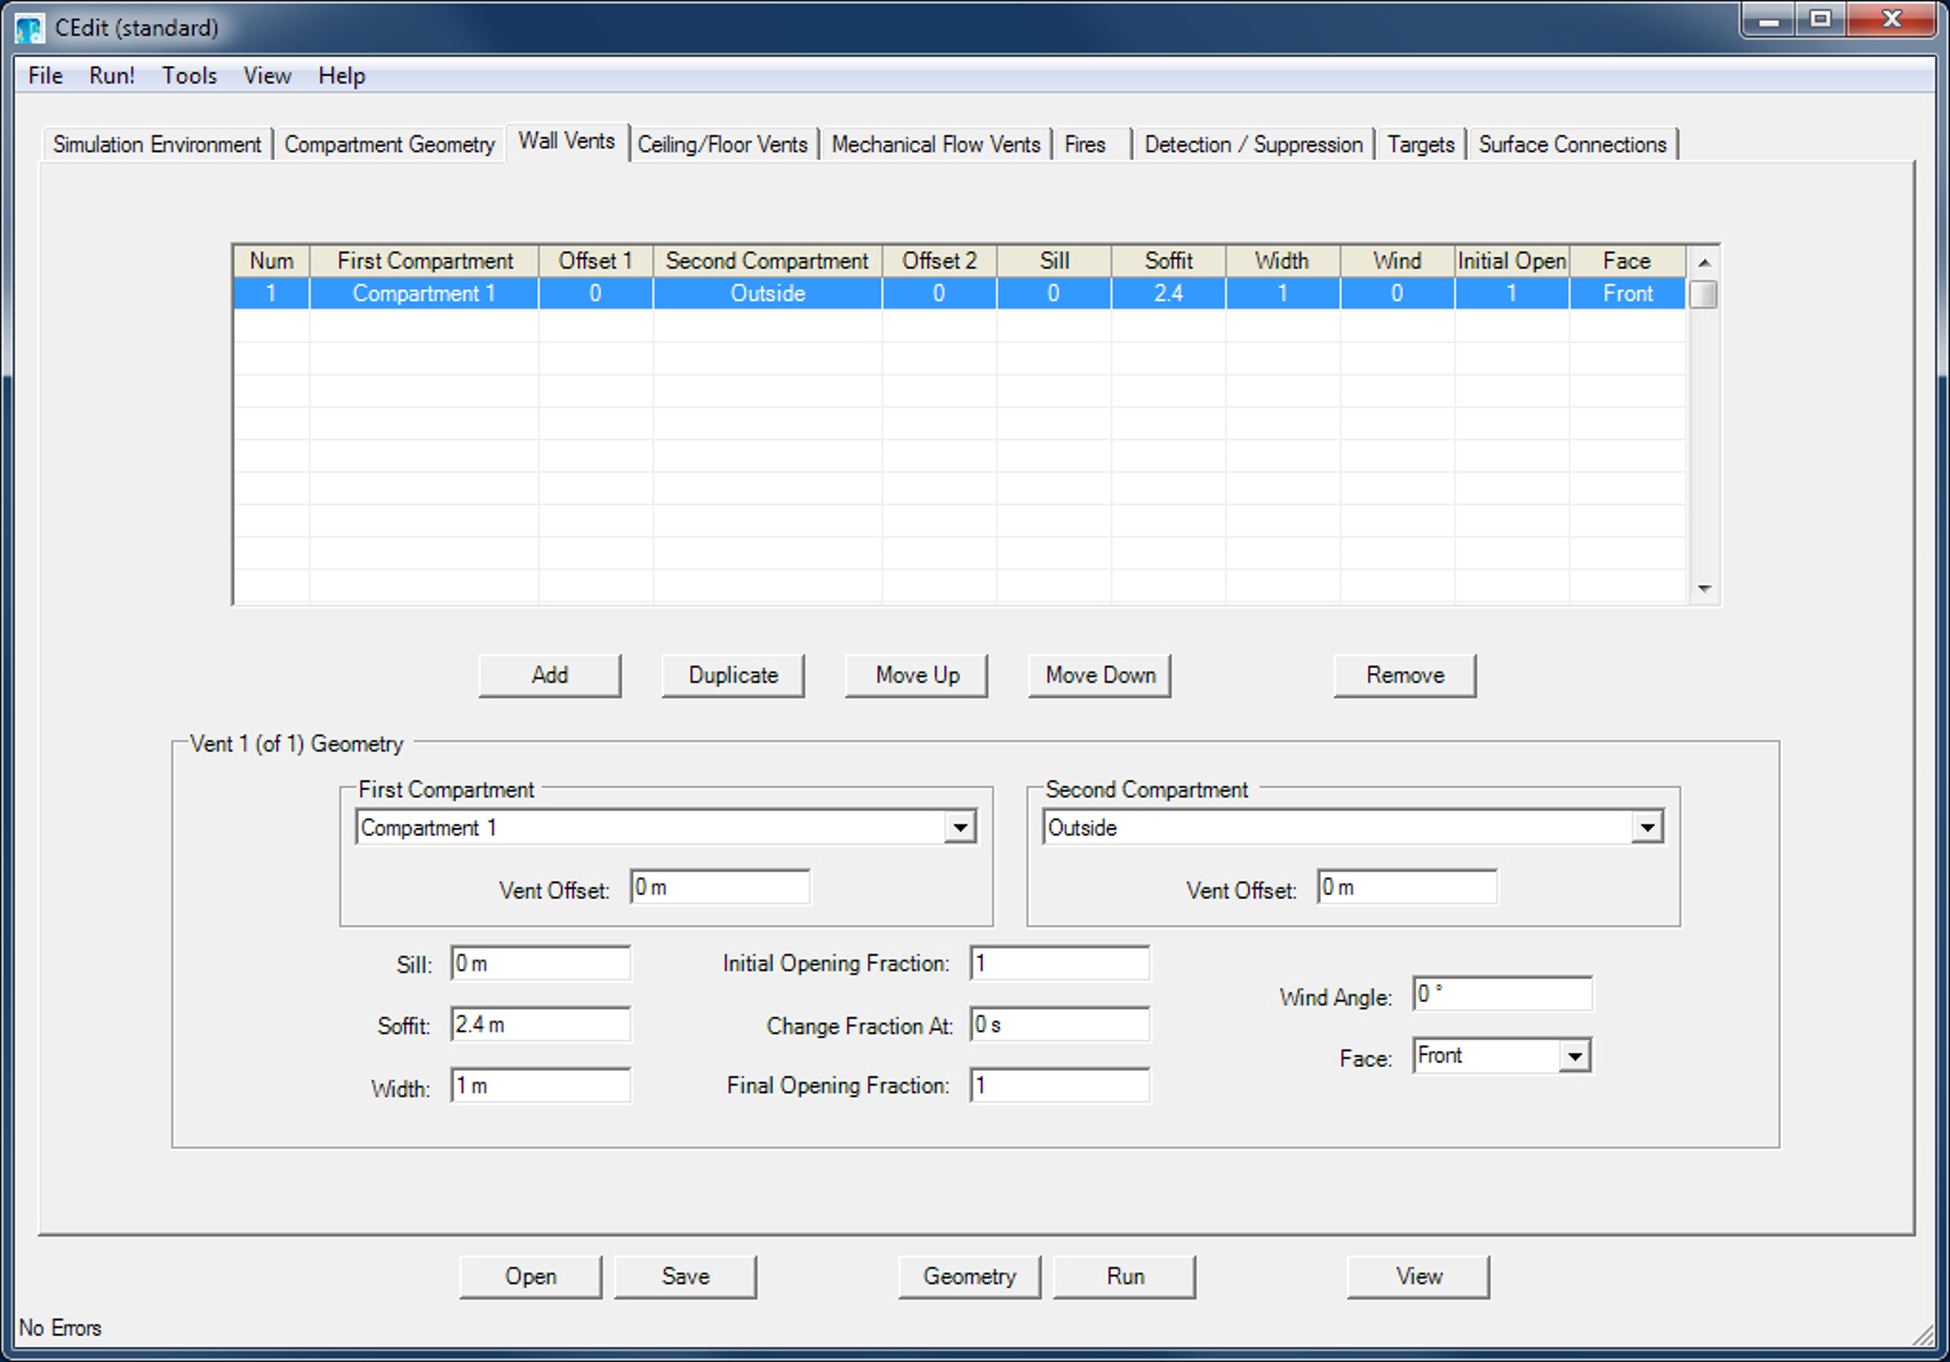
\includegraphics[width=6.5in]{FIGURES/Input_File/Natural_Flow_Tab}
\end{figure}

Most of the tabbed pages in the program are of similar design, with a summary of the defined items in table form at the top of the page, a series of buttons to add, remove, or modify the item highlighted in the summary table, and a number of individual inputs below which details all of the inputs for the item selected in the summary table. The buttons included on the horizontal flow vents page are as follows.

\begin{wrapfigure}{l}{0pt}
  
\includegraphics[width=0.781in]{FIGURES/Input_File/Add_Button}
\end{wrapfigure}

Use the Add button to create a new horizontal flow vent with default values for all entries. \\~ \\

\begin{wrapfigure}{l}{0pt}
  
\includegraphics[width=0.781in]{FIGURES/Input_File/Duplicate_Button}
\end{wrapfigure}

Use the Duplicate button to create a copy of the horizontal flow vent currently selected in the summary table at the top of the page. The new vent is added to the end of the list with the named changed to indicate it is a copy of the selected item. \\

\begin{wrapfigure}{l}{0pt}
  
\includegraphics[width=0.781in]{FIGURES/Input_File/Move_Up_Button}
\end{wrapfigure}

Use the Move Up and Move Down buttons to change the order of the list of horizontal flow vents in the summary table. This simply changes the automatically assigned vent numbers for the vents. Vents can be ordered as desired. \\~ \\

\begin{wrapfigure}{l}{0pt}
  
\includegraphics[width=0.781in]{FIGURES/Input_File/Remove_Button}
\end{wrapfigure}

Use the Remove button to delete the selected horizontal flow vent from the list of horizontal flow vents in the summary table.  Other vents are renumbered once the vent is deleted. \\~ \\

\begin{lstlisting}
HVENT,1,2,1,1,2.4,0,1,0,0,1,1
EVENT,H,1,2,1,120,1,1
\end{lstlisting}

\begin{figure}[h!]
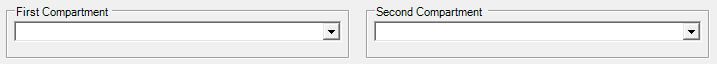
\includegraphics[width=6.5in]{FIGURES/Input_File/Compartment_From_To}
\end{figure}

\textbf{First Compartment:} First of the two compartments to be connected by a horizontal flow vent.  Compartments are numbered automatically by the input editor and by the model in the order they are read from the input data file and/or the order they appear in the summary table on the compartment geometry page. Compartment numbers begin with 1, so the first compartment is number 1, the second 2, and so forth.

\textbf{Second Compartment:} Second of the two compartments to be connected by a horizontal flow vent.  Compartments are numbered automatically by the input editor and by the model in the order they are read from the input data file and/or the order they appear in the summary table on the compartment geometry page. Compartment numbers begin with 1, so the first compartment is number 1, the second 2, and so forth.

There are also two parameters which are used to locate the compartments relative to each other. These are used to incorporate additional three dimensional information of the relative location of the vents with respect to each other. In the compartment view of CFAST, the orientation is that the rotation/translation point of the compartment is the back/bottom/left. In this view, both parameters would be with respect to the left hand side of the respective compartments. This allows the corridor filling model to incorporate a delay time for filling based on the separation between the vents. These parameters are needed only if the HALL command is used. 

\textbf{First Compartment Offset} (default units: m, Default value: 0 m): Horizontal distance between the centerline of this vent and the reference point in the first compartment.

\textbf{Second Compartment Offset } (default units: m, Default value: 0 m): Horizontal distance between the centerline of this vent and the reference point in the second compartment.

\begin{figure}[h!]
\begin{center}
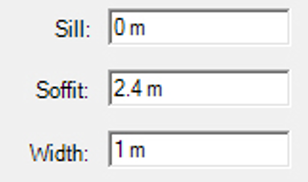
\includegraphics[width=1.1in]{FIGURES/Input_File/Vent_Size}
\end{center}
\end{figure}

\textbf{Sill} (default units: m, default value: none): Sill height is the height of the bottom of the opening relative to the floor of the compartment selected as the first compartment. 

\textbf{Soffit} (default units: m, default value: none): Position of the top of the opening relative to the floor of the compartment selected as the first compartment.   

\textbf{Width} (default units: m, default value: none): The width of the opening.

\begin{figure}[h!]
\begin{center}
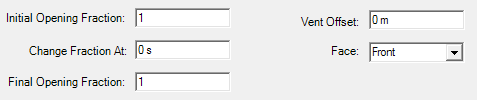
\includegraphics[width=3.1in]{FIGURES/Input_File/Vent_Open_Close}
\end{center}
\end{figure}

Horizontal flow vents may be opened or closed during the fire. The relevant CFAST keyword is EVENT. The initial format of EVENT is similar to HVENT specifying the connecting compartments and vent number.  Each EVENT line in the input file details the open/close time dependent characteristics for one horizontal flow vent by specifying a fractional value and a time.  The default is 1.0 which is a fully open vent.  A value of 0.5 would specify a vent which is halfway open.

\textbf{Initial Opening Fraction} (default value: 1): Flow through horizontal vents is calculated based on the area of the vent.  Normally, the vent is fully open.  If desired, the user may specify a fraction between 0 and 1 that allows the vent to be partially or fully closed at the beginning of the simulation.  In the model calculation, the vent width is multiplied by this fraction.  The opening fraction may be changed at any time in the simulation through the use of the EVENT command.

\textbf{Change Opening Fraction At Time}  (default units: s, default value: 0 s)  Time during the simulation at which to change the opening fraction.

\textbf{Final Opening Fraction} (default value: 1): for horizontal flow vents, the fraction specifies the fractional width opening of the vent. Fractional values must be between 0 and 1.

\textbf{Wind} (default value 0): The wind coefficient is the cosine of the angle between the wind vector and the vent opening.  This applies only to vents which connect to the outside.  The range of values is -1.0 to 1.0.  In the input editor, this is specified as the angle between the face of the vent and the wind direction.

\textbf{Face:} For visualization, FACE specifies which wall the vent will be displayed on in smokeview.  Choices are Front, Rear, Right, Left and are relative to the X-Z plane.

\begin{itemize}
\item The soffit and sill specifications are with respect to the first compartment specified and is not necessarily symmetric since the elevation of the second compartment may be different than the first.  Reversing the order of the compartment designations does make a difference.
\end{itemize}

\subsection{Defining Natural Flow Connection Through Ceiling and Floor Openings}

This section of the input data file describes these vertical flow openings. Examples of these openings are scuddles in a ship, or a hole in the roof of a residence. Combined buoyancy- and pressure-driven (i.e., forced) flow through a vertical flow vent is possible when the connected spaces adjacent to the vent are filled with gases of different density in an unstable configuration, with the density of the top space larger than that of the bottom space. With a moderate cross-vent pressure difference, the instability leads to a bi-directional flow between the two spaces. For relatively large cross-vent pressure difference the flow through the vent is unidirectional, from the high- to the low-pressure space. 
Connections can exist between compartments or between a compartment and the outdoors. Openings to the outside are included as openings to a compartment with a number one greater than the number of compartments defined in the scenario.  These connections are described by the VVENT keyword. Each VVENT line in the input file describes one vertical vent.  There are four parameters which include each of the connected compartments, the shape of the opening, and the effective area of the vent.

\begin{figure}[h!]
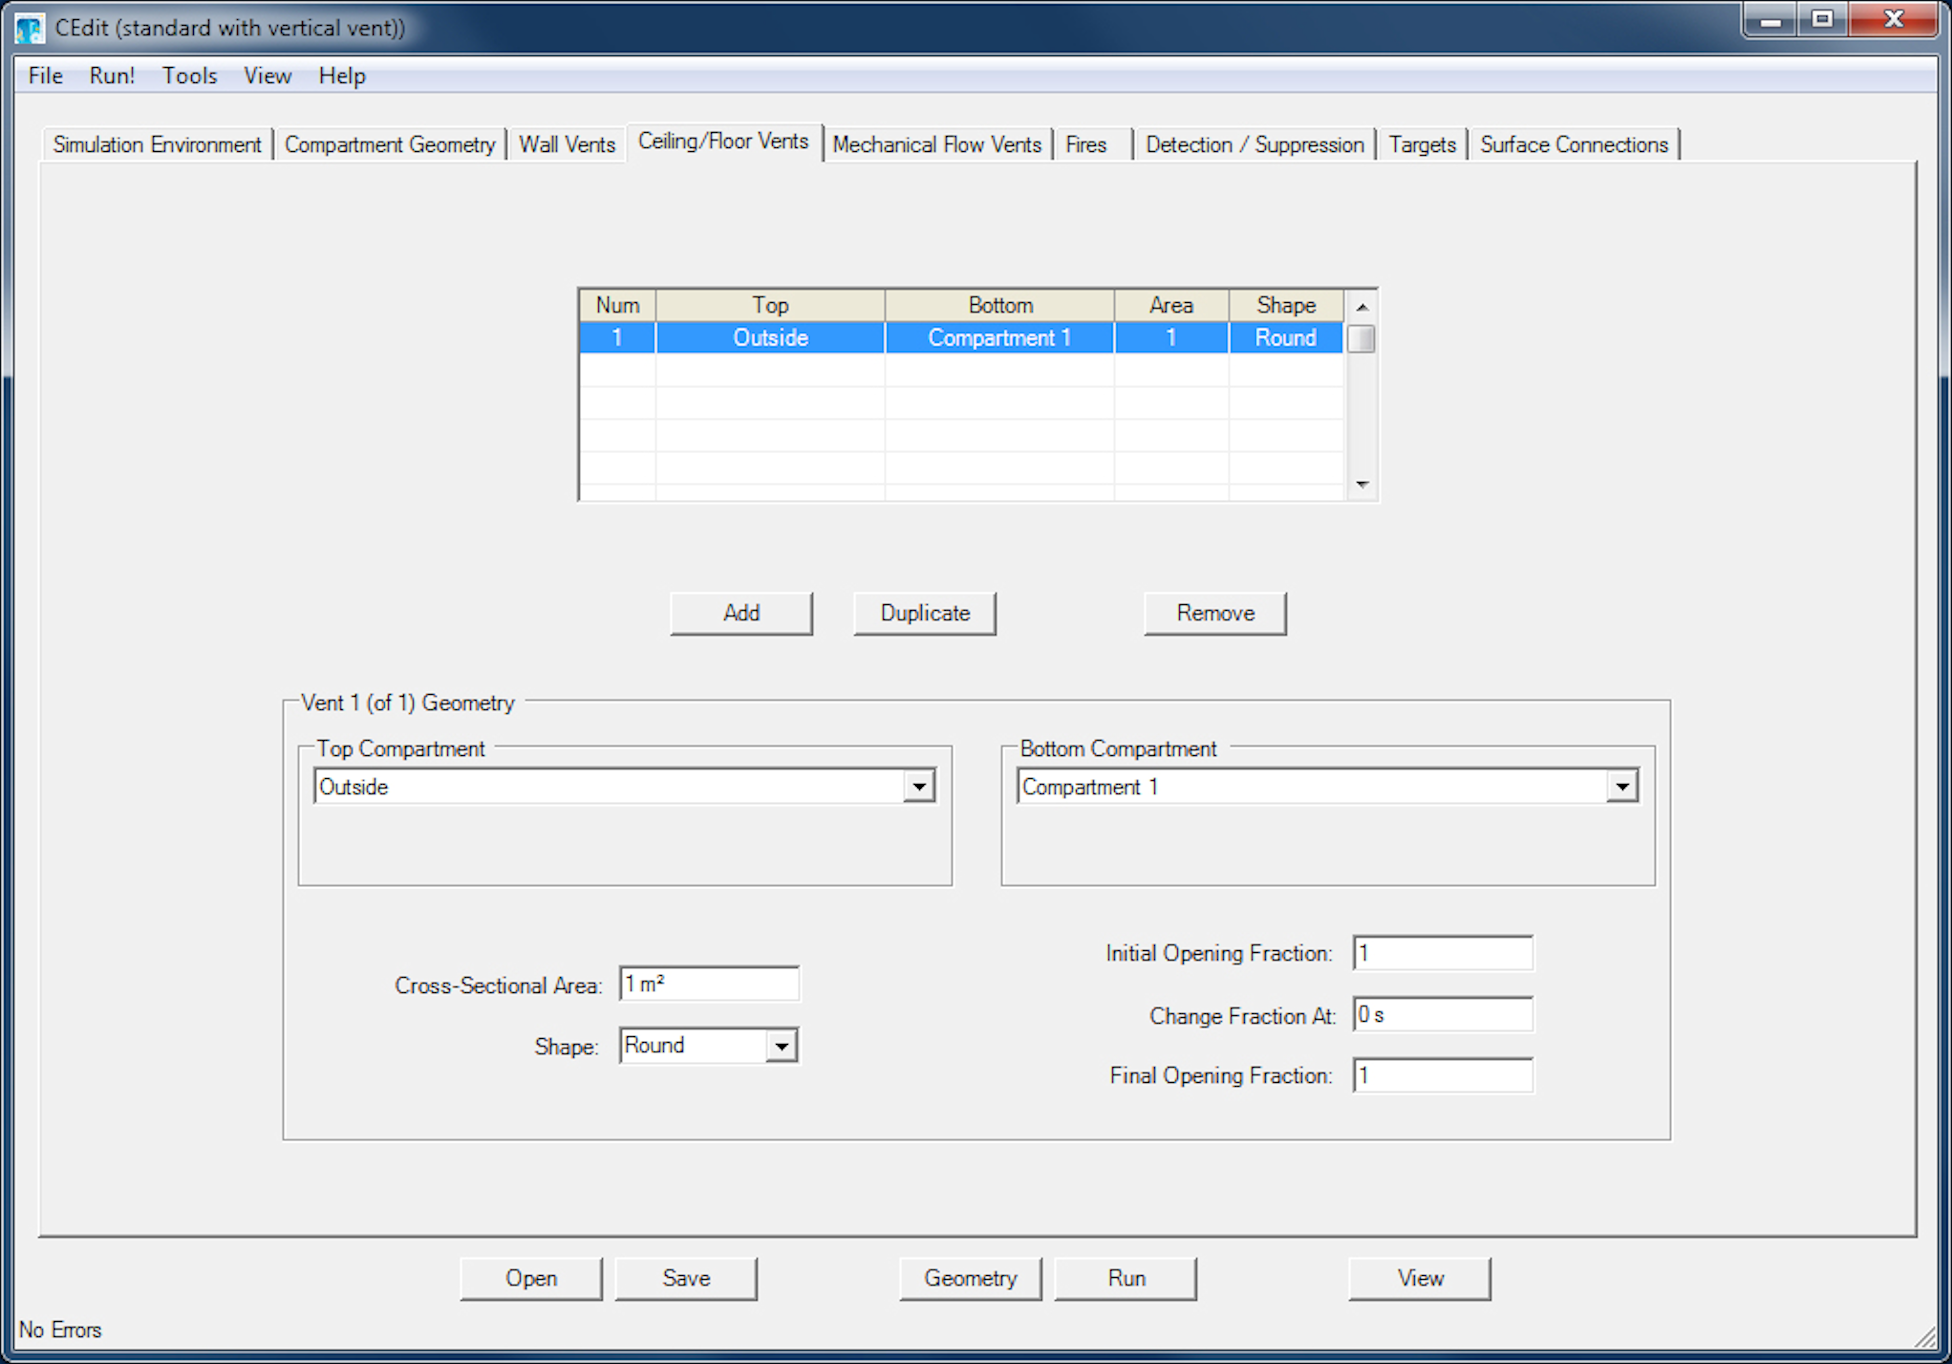
\includegraphics[width=6.5in]{FIGURES/Input_File/Vertical_Flow_Tab}
\end{figure}
 
Most of the tabbed pages in the program are of similar design, with a summary of the defined items in table form at the top of the page, a series of buttons to add, remove, or modify the item highlighted in the summary table, and a number of individual inputs below which details all of the inputs for the item selected in the summary table. The buttons included on the vertical flow vents page are as follows.

\begin{wrapfigure}{l}{0pt}
  
\includegraphics[width=0.781in]{FIGURES/Input_File/Add_Button}
\end{wrapfigure}

Use the Add button to create a new vertical flow vent with default values for all entries. \\~ \\

\begin{wrapfigure}{l}{0pt}
  
\includegraphics[width=0.781in]{FIGURES/Input_File/Duplicate_Button}
\end{wrapfigure}

Use the Duplicate button to create a copy of the vertical flow vent currently selected in the summary table at the top of the page. The new vent is added to the end of the list with the named changed to indicate it is a copy of the selected item. \\

\begin{wrapfigure}{l}{0pt}
  
\includegraphics[width=0.781in]{FIGURES/Input_File/Remove_Button}
\end{wrapfigure}

Use the Remove button to delete the selected vertical flow vent from the list of vertical flow vents in the summary table.  Other vents are renumbered once the vent is deleted. \\~ \\

\begin{lstlisting}
VVENT,2,1,2.44,2,1
EVENT,V,1,2,1,120,1,1
\end{lstlisting}

\textbf{Top Compartment:} The top or first of the two compartments to be connected by a vertical flow vent. The vent is through the floor of this compartment.  Compartments are numbered automatically by the input editor and by the model in the order that they are read from the input data file and/or the order they appear in the summary table on the compartment geometry page. Compartment numbers begin with 1, so the first compartment is number 1, the second 2, and so forth.

\textbf{Bottom Compartment:} The bottom or second of the two compartments to be connected by a horizontal flow vent. The vent is through the ceiling of this compartment. Compartments are numbered automatically by the input editor and by the model in the order they are read from the input data file and/or the order they appear in the summary table on the compartment geometry page. Compartment numbers begin with 1, so the first compartment is number 1, the second 2, and so forth.

\textbf{Cross-sectional Area} (default units: m$^2$, default value: none): specifies the cross-sectional area of the vent connecting the two compartments.

\textbf{Shape:} The shape factor is 1 for circular openings and 2 for square openings.

\textbf{Initial Opening Fraction:} Flow through vertical vents is calculated based on the area of the vent.  Normally, the vent is fully open.  If desired, the user may specify a fraction between 0 and 1 that allows the vent to be partially or fully closed at the beginning of the simulation.  In the model calculation, the vent area is multiplied by this fraction.  The opening fraction may be changed at any time in the simulation through the use of the EVENT command.

\textbf{Change Opening Fraction At Time} (default units: s, default value: 0 s): Time during the simulation at which to change the opening fraction.

\textbf{Final Opening Fraction:} for vertical flow vents, the fraction specifies the fractional cross-sectional area of the vent. Fractional values must be between 0 and 1.

\begin{itemize}
\item Although obvious, note that the top or first compartment must be the compartment on top of the bottom or second compartment.
\item CFAST allows only a single connection between any pair of compartments included in a simulation. This limitation is based on the implementation of the vertical flow algorithm in CFAST and on the validation efforts for the original algorithm development  which only studied a single opening between connected compartments.
\item Vertical connections can only be created between compartments that could be physically stacked based on specified floor and ceiling elevations for the compartments.  Some overlap between the absolute floor height of one compartment and the absolute ceiling height of another compartment is allowed.  However, whether the compartments are stacked or overlap somewhat, the ceiling/floor absolute elevations must be within 0.01 m of each other. The check is not done when the connection is to the outside.
\end{itemize}

\subsection{Defining Mechanical Ventilation Connections}

Fan-duct systems are commonly used in buildings for heating, ventilation, air conditioning, pressurization, and exhaust. Generally, systems that maintain comfortable conditions have either one or two fans.  Residences often have a systems with a single fan. Further information about these systems is presented in  Klote and Milke \cite{Klote:2002} and the American Society of Heating, Refrigerating and Air Conditioning Engineers \cite{ASHRAE:2001}.

\begin{figure}[h!]
\begin{center}
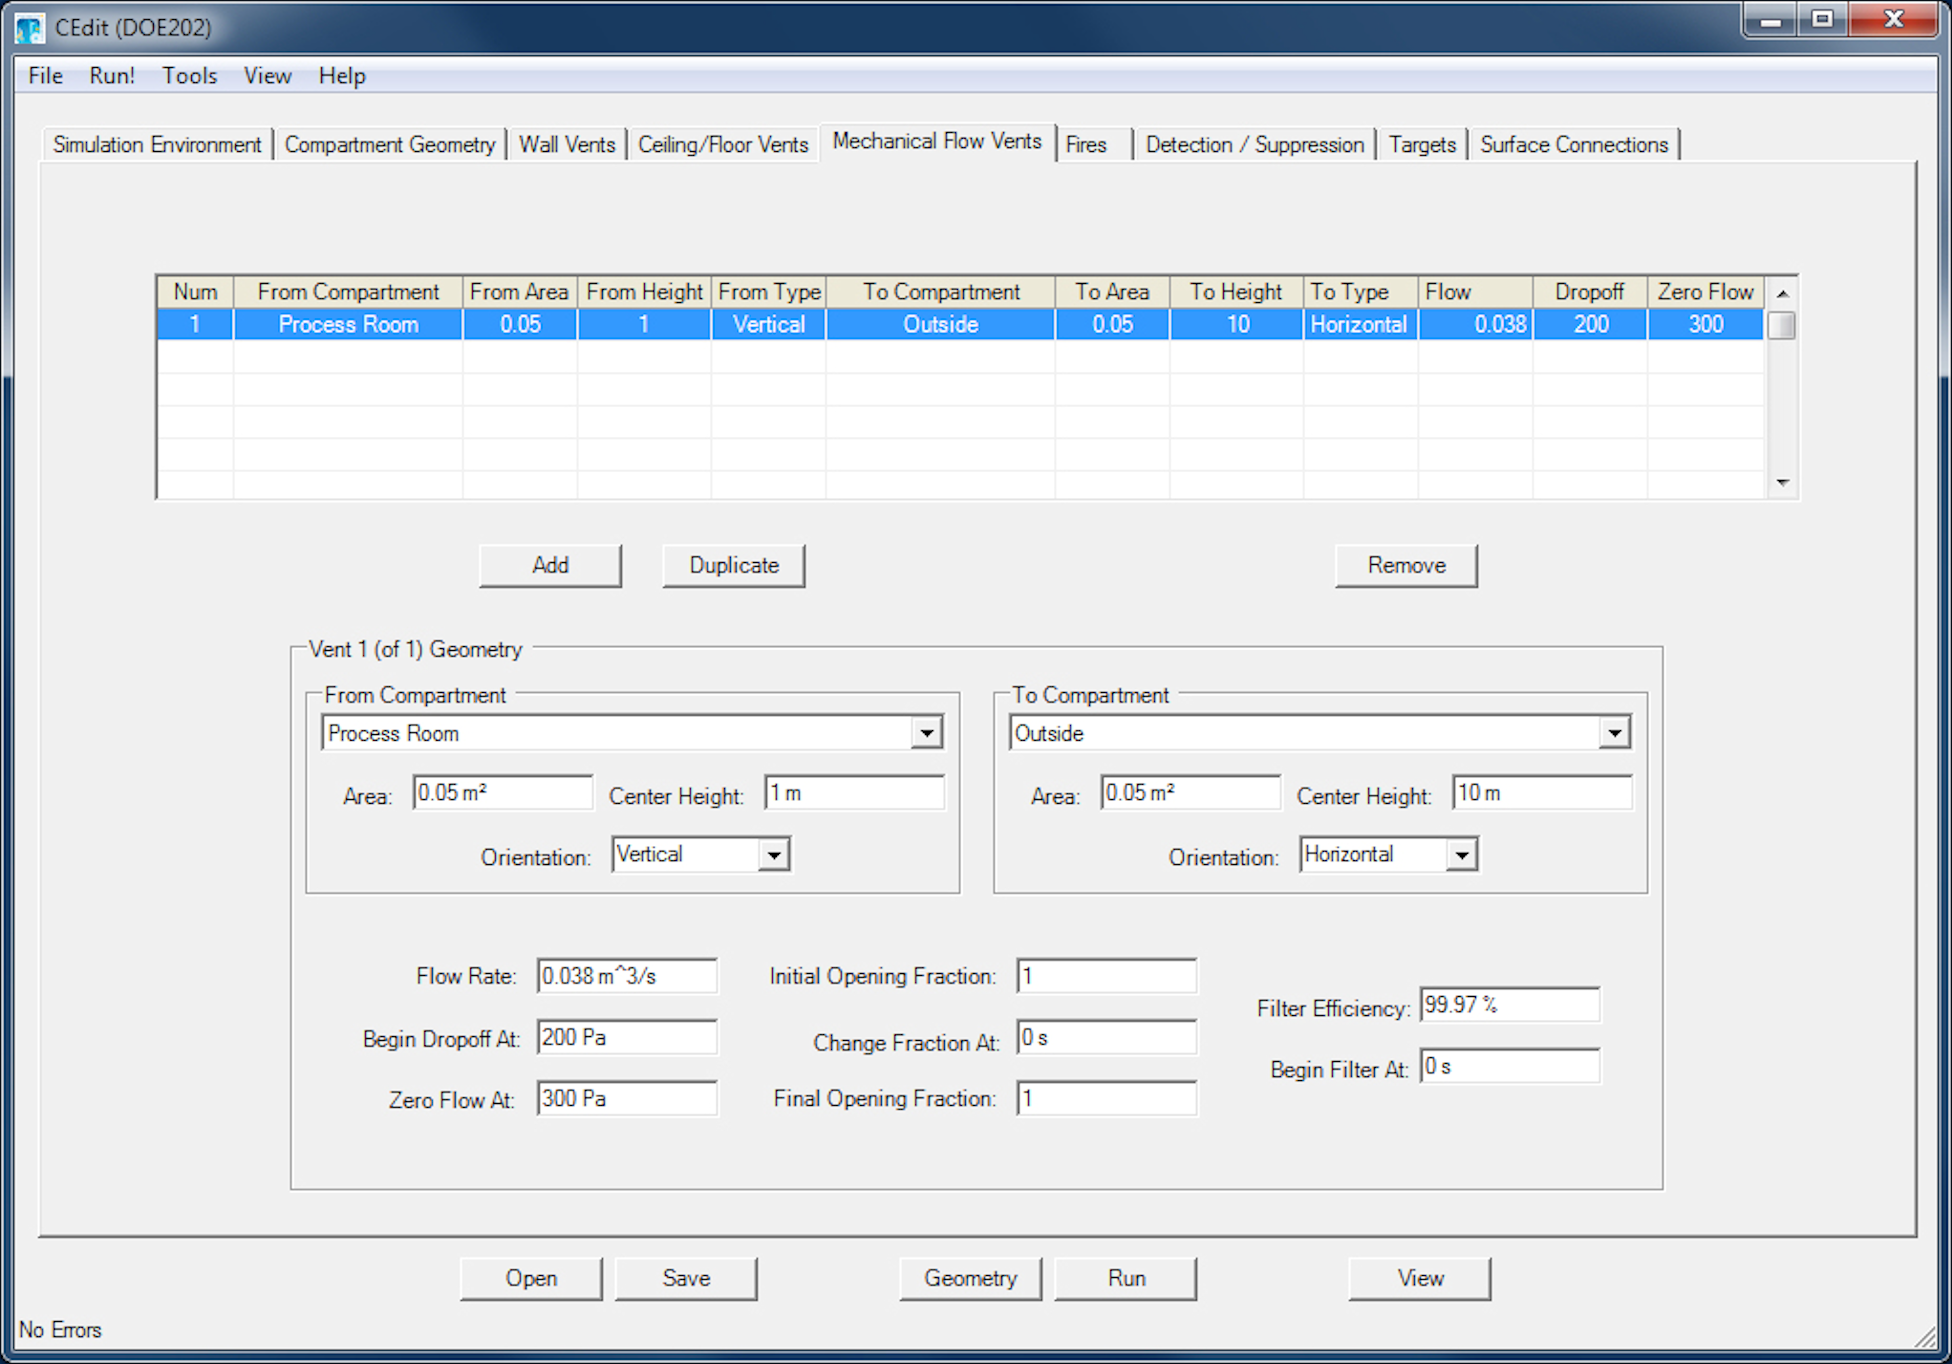
\includegraphics[width=6.5in]{FIGURES/Input_File/Mechanical_Vent_Tab}
\end{center}
\end{figure}

The model for mechanical ventilation used in CFAST is based on the theory of networks and is based on the model developed by Klote \cite{Klote:1988a}.  This is a simplified form of Kirchoff's law which says that flow into a node must be balanced by flow out of the node. The equations used describe the relationship between the pressure drop across a duct, the resistance of a duct, and the mass flow.  The pressure can be changed by conditions in a compartment, or a fan in line in the duct system.  Resistance arises from the finite size of ducts, roughness on duct surfaces, bends and joints. In CFAST, default values are used for the duct properties, and thus mechanical ventilation connections are simply described by the connections to the two compartments and a fan whose throughput is a constant volumetric flow up to a user-specified pressure drop across the fan, dropping to zero at high backwards pressure on the fan.

Most of the tabbed pages in the program are of similar design, with a summary of the defined items in table form at the top of the page, a series of buttons to add, remove, or modify the item highlighted in the summary table, and a number of individual inputs below which details all of the inputs for the item selected in the summary table. The buttons included on the mechanical flow vents page are as follows.

\begin{wrapfigure}{l}{0pt}
  
\includegraphics[width=0.781in]{FIGURES/Input_File/Add_Button}
\end{wrapfigure}

Use the Add button to create a new mechanical flow vent with default values for all entries. \\~ \\

\begin{wrapfigure}{l}{0pt}
  
\includegraphics[width=0.781in]{FIGURES/Input_File/Duplicate_Button}
\end{wrapfigure}

Use the Duplicate button to create a copy of the mechanical flow vent currently selected in the summary table at the top of the page. The new vent is added to the end of the list with the named changed to indicate it is a copy of the selected item. \\

\begin{wrapfigure}{l}{0pt}
  
\includegraphics[width=0.781in]{FIGURES/Input_File/Remove_Button}
\end{wrapfigure}

Use the Remove button to delete the selected mechanical flow vent from the list of vertical flow vents in the summary table.  Other vents are renumbered once the vent is deleted. \\~ \\

\begin{lstlisting}
MVENT,2,3,1,V,0.6,0.4225,V,0.75,0.0731,0.167,2000,3000,1
\end{lstlisting}

\begin{figure}[h!]
\begin{center}
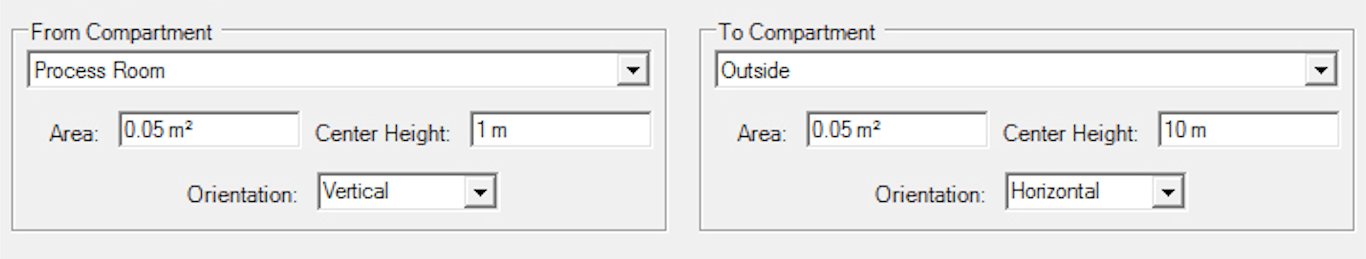
\includegraphics[width=4.553in]{FIGURES/Input_File/Mechanical_Vent_From_To}
\end{center}
\end{figure}
 
\textbf{From Compartment:} The first compartment to which the mechanical ventilation system diffuser is connected. Fan flow is from this compartment.  Compartments are numbered automatically by the input editor and by the model in the order they are read from the input data file and/or the order they appear in the summary table on the compartment geometry page. Compartment numbers begin with 1, so the first compartment is number 1, the second 2, and so forth.

\textbf{From Compartment Area} (default units: m$^2$, default value: none): Cross-sectional area of the opening into the compartment. The area will be truncated if the midpoint (height) is set such that the height plus or minus the effective length is above the compartment ceiling or below the floor.

\textbf{From Compartment Height} (default units: m, default value: none): Height of the duct opening above the floor of the compartment measured from the midpoint of the register.

\textbf{From Compartment Orientation:} The orientation of the diffuser relative to the floor of the compartment.  A horizontal diffuser implies vertical flow through the ceiling or floor of the compartment.  A vertical diffuser implies horizontal flow through a wall of the compartment.

\textbf{To Compartment:} The bottom or second of the two compartments to be connected by a horizontal flow vent. The vent is through the ceiling of this compartment. Compartments are numbered automatically by the input editor and by the model in the order they are read from the input data file and/or the order they appear in the summary table on the compartment geometry page. Compartment numbers begin with 1, so the first compartment is number 1, the second 2, and so forth.

\textbf{To Compartment Area} (default units: m$^2$, default value: none): Cross-sectional area of the opening into the compartment. The area will be truncated if the midpoint (height) is set such that the height plus or minus the effective length is above the compartment ceiling or below the floor.

\textbf{To Compartment Height} (default units: m, default value: none): Height of the duct opening above the floor of the compartment measured from the midpoint of the register.

\textbf{To Compartment Orientation:} The orientation of the diffuser relative to the floor of the compartment.  A horizontal diffuser implies vertical flow through the ceiling or floor of the compartment.  A vertical diffuser implies horizontal flow through a wall of the compartment.

\begin{figure}[h!]
\begin{center}
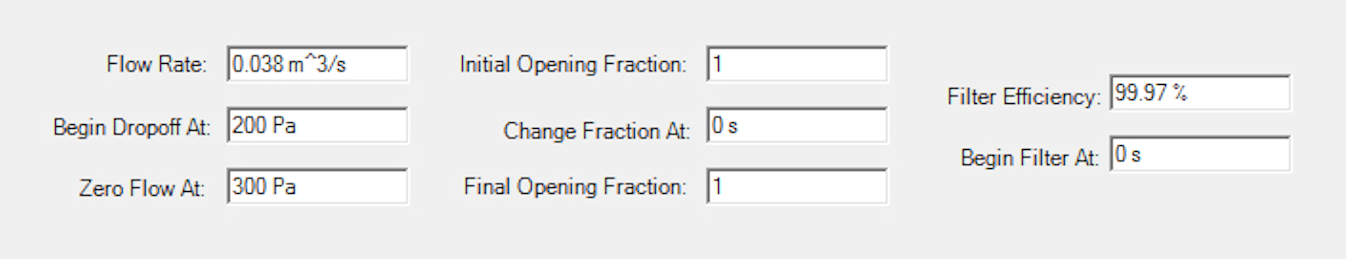
\includegraphics[width=4.487in]{FIGURES/Input_File/Mechanical_Vent_Flowrate}
\end{center}
\end{figure}

\textbf{Flow Rate} (default units: m$^3$/s, default value: none): Constant flow rate of the forced-air flow from the first compartment to the second compartment.

\textbf{Begin Drop Off Pressure} (default units: Pa, default value: 200 Pa): The description of the fan includes a drop off in flow beginning at a pressure specified by the user.  Above this pressure drop, the flow gradually drops to zero flow.

\textbf{Zero Flow Pressure} (default units: Pa, default value: 300 Pa): Specifies the pressure above which the flow through the mechanical ventilation connection is zero.

\textbf{Initial Opening Fraction:} Flow through mechanical vents is calculated based on the area of the vent.  Normally, the vent is fully open.  If desired, the user may specify a fraction between 0 and 1 that allows the vent to be partially or fully closed at the beginning of the simulation.  In the model calculation, the fan flow rate is multiplied by this fraction.  The opening fraction may be changed at any time in the simulation through the use of the EVENT command.

\textbf{Change Opening Fraction At Time} (default units: s, default value: none): Time during the simulation at which to change the opening fraction.

\textbf{Final Opening Fraction:} for mechanical flow vents, the fraction specifies the fractional fan flow rate for the vent. Fractional values must be between 0 and 1.

\textbf{Filter Efficiency} (default units:~\%, default value: none): Flow through mechanical vents may include filtering that removes a user-specified portion of soot and trace species mass from the flow through the vent.  By default, there is no filtering applied, that is all of the soot and trace species mass in the vent flow is passed through the vent. Within the user interface, this is specified as a filter efficiency of 0~\%.  If desired, the user may specify the fraction of the soot and trace species mass to be removed as a percentage.

\textbf{Begin Filtering At Time} (default units: s, default value: none): Time during the simulation at which the mechanical vent filtering begins.

\begin{itemize}
\item CFAST does not include provisions for reverse flow through a fan. Calibration for backward flow is not provided by fan manufacturers, so the equations incorporated in CFAST do not allow for such flow. The problem is simply that in this flow regime, the fan has stalled, and likely will soon fail. 
\item If the simulation includes mechanical ventilation filtering, care should be taken in choosing trace species production rates to insure the production rate is small compared to the total pyrolysis rate.  This will allow appropriate conservation of mass in the solution of the system of differential equation.  For large production rates of trace species, scaling factors can be used (e.g., divide by 1000) for the trace species production rate to reduce the relative magnitude compared to the pyrolysis rate.  For analysis, the resulting trace species in compartments and filters can be converted back to original units multiplying by the scaling factor used.
\end{itemize}

\newpage
\section{Prescribing Fires}

A simulated fire in CFAST is implemented as a source of fuel mass which is released at a prescribed rate (the pyrolysis rate). Energy is released by the fuel and combustion products are created as it burns. In the fire, species production is calculated based on production yields prescribed by the user. In addition, the pyrolysis rate and resulting energy and species generation may be limited by the oxygen available for combustion. When sufficient oxygen is available for combustion, the heat release rate for the constrained fire is the same as for the unconstrained fire.

The model can simulate multiple fires in one or more compartments of the building.  These fires are treated as totally separate entities, with no interaction of the plumes. These fires are generally referred to as “objects” and can be ignited at a prescribed time, temperature or heat flux.

CFAST does not include a pyrolysis model to pre¬dict fire growth. Rather, pyrolysis rates for each fire are prescribed by the user.  ¬While this approach does not directly account for increased pyrolysis due to radiative feedback from the flame or com¬part¬ment, in theory these effects could be prescribed by the user as described in this section.  In an actual fire, this is an important consideration, and the specification used should consider the experimental conditions as closely as possible.

A fire releases energy based on the pyrolysis of fuel, but may be constrained by the oxygen available for combustion depending on the compartment conditions. Complete burning will take place only where there is suffi¬cient oxygen.  When insufficient oxygen is entrained into the fire plume, unburned fuel will be transported from zone to zone until there is sufficient oxygen and a high enough temperature to support combustion.  In general, CFAST uses a simple definition of a combustion reaction that includes major products of combustion for hydrocarbon fuels:
\be  \mathrm{C_{n_\C}H_{n_H}O_{n_O}N_{n_N}Cl_{n_{Cl}}} +  \nu_\OTWO \, \mathrm{O_2}  \rightarrow  \nu_\COTWO \, \mathrm{CO_2} + \nu_\HTWOO \, \mathrm{H_2O} + \nu_\CO \, \mathrm{CO} +
     \nu_\So \, \mathrm{Soot}  + \nu_\HCl \mathrm{HCl} + \nu_\HCN \mathrm{HCN} \label{stoich} \ee
assuming that all the nitrogen and chlorine in the fuel are converted to HCN and HCl. The stoichiometric coefficients $\nu_\So$, $\nu_\CO$, etc. represent appropriate molar ratios for a stoichiometric balance of the equation. For complete combustion of the simplest hydrocarbon fuel, methane reacts with oxygen to form carbon dioxide and water. The only inputs required are the fuel composition, heat release rate, and heat of combustion. For fuels that contain oxygen, nitrogen, or chlorine, the reaction becomes more complex. Stoichiometry is used to insure conservation of mass and elements in the reaction. The species which are calculated are oxygen, carbon dioxide, carbon monoxide, water, total unburned hydrocarbons (tuhc), and soot. Gaseous nitrogen is included, but only acts as a diluent. 

Production of hydrogen cyanide and hydrogen chloride are tracked solely based on user prescribed yields.  

The heat release rate for a constrained fire may be reduced below its prescribed value based upon the oxygen available for combustion. For the constrained fire, the burning rate may be less than the pyrolysis rate and cannot be simplified as in the case of the unconstrained fire. As fuel and oxygen are consumed, heat is released and various products of combustion are formed.

For a constrained fire, the heat release rate is limited by available oxygen. This limit is applied in three places: The first is burning in the portion of the plume which is in the lower layer of the room of fire origin; the second is the portion of the plume in the upper layer, also in the room of origin; the third is in the vent flow which entrains air from a lower layer into an upper layer in an adjacent compartment. The unburned hydrocarbons are tracked in this model. Combustion of CO to CO$_2$ is not included in the model. Actual combustion chemistry is not considered in CFAST due to the complexities associated with detailed kinetics and transport.

There are two calculations involving radiation in this model. One is for energy balance and is based on broadband radiation absorption. The amount of radiation absorbed in sensitive to the species present, specifically water vapor, soot and carbon dioxide. The other is for visibility of egress signs. This calculation is based solely on the soot volume fraction and is reported as optical depth (per meter). The conversion factor is based on the recent work by Mulholland and Croarkin \cite{Mullholland:2000}. The value for converting mass density in kg/m3 to optical depth is 3817 m$^2$/kg. The value reported is intended specifically for assessing the visibility of egress signs, based on the work of Jin \cite{Jin:1979}.  It is not applicable to the far blue or red regions of the spectrum and so should not be used for assessing optical detection of fires through smoke.

\begin{figure}[h!]
\begin{center}
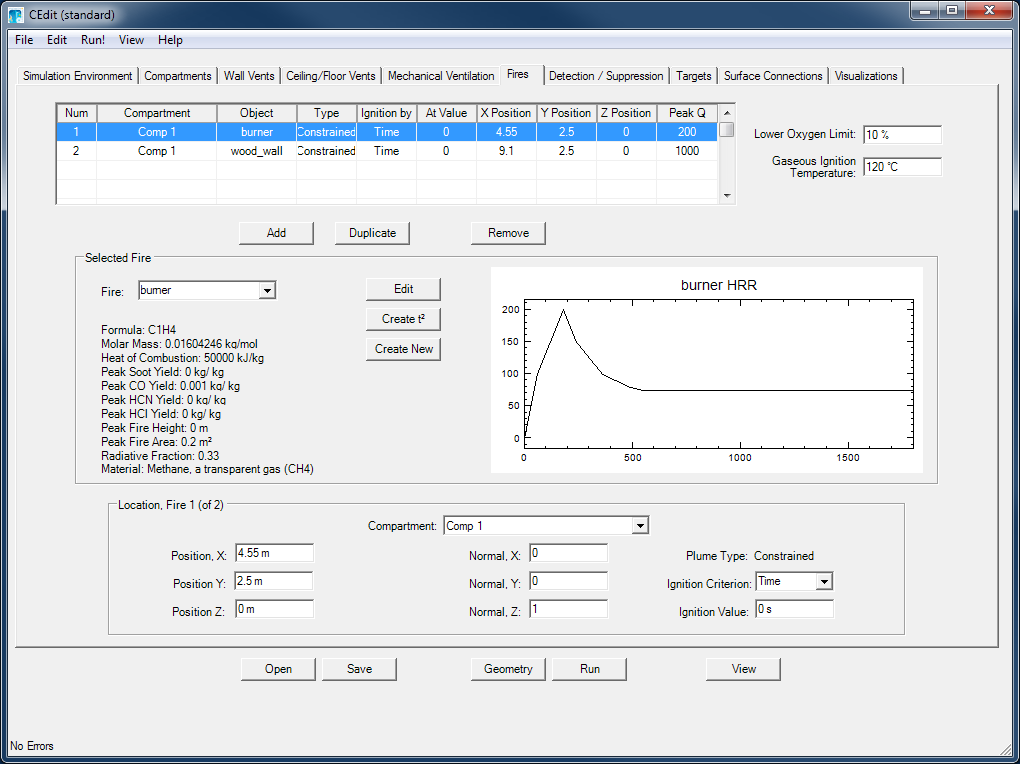
\includegraphics[width=6.5in]{FIGURES/Input_File/Fire_Tab}
\end{center}
\end{figure}
 
Most of the tabbed pages in the program are of similar design, with a summary of the defined items in table form at the top of the page, a series of buttons to add, remove, or modify the item highlighted in the summary table, and a number of individual inputs below which details all of the inputs for the item selected in the summary table. The buttons included on the fires page are as follows.


\begin{wrapfigure}{l}{0pt}
  
\includegraphics[width=0.781in]{FIGURES/Input_File/Add_Button}
\end{wrapfigure}

Use the Add button to create a new fire with default values for all entries. \\~ \\

\begin{wrapfigure}{l}{0pt}
  
\includegraphics[width=0.781in]{FIGURES/Input_File/Duplicate_Button}
\end{wrapfigure}

Use the Duplicate button to create a copy of the fire currently selected in the summary table at the top of the page. The new fire is added to the end of the list with the named changed to indicate it is a copy of the selected item. \\

\begin{wrapfigure}{l}{0pt}
  
\includegraphics[width=0.781in]{FIGURES/Input_File/Remove_Button}
\end{wrapfigure}

Use the Remove button to delete the selected fire from the list of fires in the summary table.  Other fires are renumbered once the fire is deleted. \\~ \\

\begin{lstlisting}
!!Wood_Wall
FIRE,1,4.55,2.5,0,1,1,0,0,0,1,Wood_Wall
CHEMI,1,4,0,0,0,0.33,1.81E+07,HARDWOOD
TIME,0,8000
HRR,0,1000000
SOOT,0.02,0.02
CO,0.02,0.02
TRACE,0,0
AREA,0.05,9
HEIGH,0,3
\end{lstlisting}

\subsection{Global Fire Inputs}

Three inputs on the Fire Tab are global, that is, they apply to all fires included in a simulation.

\begin{wrapfigure}{l}{0pt}
  
\includegraphics[width=2.313in]{FIGURES/Input_File/Ceiling_Jet}
\end{wrapfigure}

\textbf{Ceiling Jet}: If the fire is large enough, the plume from the fire will penetrate the upper layer, impinge on the ceiling surface, and increase the convective heat transfer to the ceiling or increase the temperature nearby targets or detectors near the ceiling.  CFAST includes an algorithm to account for some of these effects.  Details of the inputs are included in the section on ceiling jets included in the Special Features chapter, below.

\begin{wrapfigure}{r}{0pt}
  
\includegraphics[width=2.240in]{FIGURES/Input_File/LOL}
\end{wrapfigure}

\textbf{Lower Oxygen Limit} (default units: \%, default value: 10~\%):  In the CFAST model, a limit is incorporated by limiting the burning rate as the oxygen level decreases until a ``lower oxygen limit'' (LOL) is reached. The lower oxygen limit is incorporated through a smooth decrease in the burning rate near the limit. Normally, this value would not be changed by the user.

\begin{wrapfigure}{l}{0pt}
  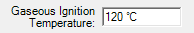
\includegraphics[width=2.021in]{FIGURES/Input_File/Gaseous_Ignition_Temperature}
\end{wrapfigure}

\textbf{Gaseous Ignition Temperature} (default units: \degc, default value: ambient temperature plus 100 K): The lower temperature limit on the burning of fuel in a gas layer. Since CFAST does not support a combustion kinetics model, this is the algorithm used for fires out of vents.  Normally, this value would not be changed by the user.

\subsection{Defining Individual Fires}

Fires in CFAST are defined as a series of individual fire objects which are then placed as desired in compartments in a simulation.

Each fire object defines the time dependent variables of the fire are described by the mass loss rate, rate of heat release, fuel height, and fuel area inputs.  Species production rates are specified in a manner similar to the fire, entering the rates as a series of points with respect to time.  The species which are followed by CFAST are: carbon dioxide, carbon monoxide, hydrogen cyanide, hydrogen chloride, nitrogen, oxygen, soot, total unburned hydrocarbons and water. There is a separate calculation of the concentration-time product Ct. Finally, a user-specified trace species can be specified to follow the transport that results from fire-induced flow for an arbitrary species. This may be of particular interest for radiological releases \cite{Jones:2008}, but may be useful for any trace amounts released by a fire.

\begin{figure}[h!]
\begin{center}
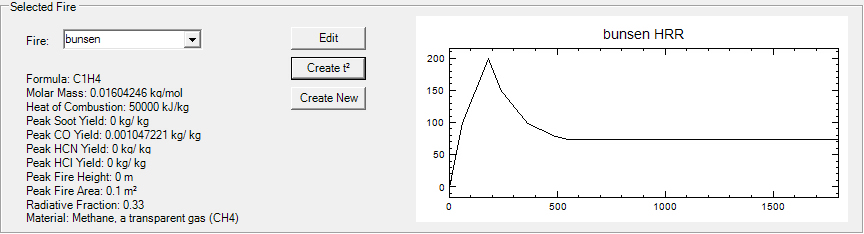
\includegraphics[width=6.5in]{FIGURES/Input_File/Fire_Object_Plot}
\end{center}
\end{figure}


\begin{wrapfigure}{r}{0pt}
  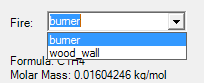
\includegraphics[width=1.948in]{FIGURES/Input_File/Fire_Pulldown}
\end{wrapfigure}

Each fire object is defined in a separate comma-separated spreadsheet file with an extension of ``.o' and saved in the CFAST input file for the current simulation. As many fire objects as desired may be defined by the user.  At least one fire in the simulation should ignite at a user-specified time.  Other fire objects can ignite based on time, temperature or heat flux conditions. A pull-down allows the user to select one of the predifined fire objects to place in the chosen compartment. \\~ \\~ \\

\begin{wrapfigure}{l}{0pt}
  
\includegraphics[width=0.781in]{FIGURES/Input_File/Edit_Button}
\end{wrapfigure}

Use the Edit button to edit the currently selected fire object. Fire Objects can also be changed from the Tools menu. A separate window allows the user to view or change any of the available fire objects. Details of fire inputs for a fire is included below.

\begin{wrapfigure}{l}{0pt}
  
\includegraphics[width=0.781in]{FIGURES/Input_File/Create_t2_Button}
\end{wrapfigure}

Use the Create t$^2$ button to create a new fire object with a heat release rate specified by the user in the form of a t-squared fire.  For a wide range of fires, the fire growth can be accurately represented with a power law relation of the form $\dQ=\alpha t^2$  where $\dQ$  is the heat release rate of the fire, $\alpha$ is the fire intensity coefficient, and $t$ is time \cite{Schifiliti:2002}. A set of specific t-squared fires labeled slow, medium, and fast, with fire intensity coefficients ($\alpha$) such that the fires reached 1054 kW (1000 BTU/s) in 600 s, 300 s, and 150 s, respectively were proposed for design of fire detection systems .  Later, these specific growth curves and a fourth called "Ultra-fast" which reaches 1054 kW in 75 s, gained favor in general fire protection applications. A separate window allows the user to define the t-squared fire. Details of the inputs for a t-squared fire is included below.
 

\begin{wrapfigure}{l}{0pt}
  
\includegraphics[width=0.781in]{FIGURES/Input_File/Create_New_Button}
\end{wrapfigure}

Use the Create New button to create a new fire object with default values for all entries.  No time-dependent values are included in the new fire.

\begin{figure}[h!]
\begin{center}
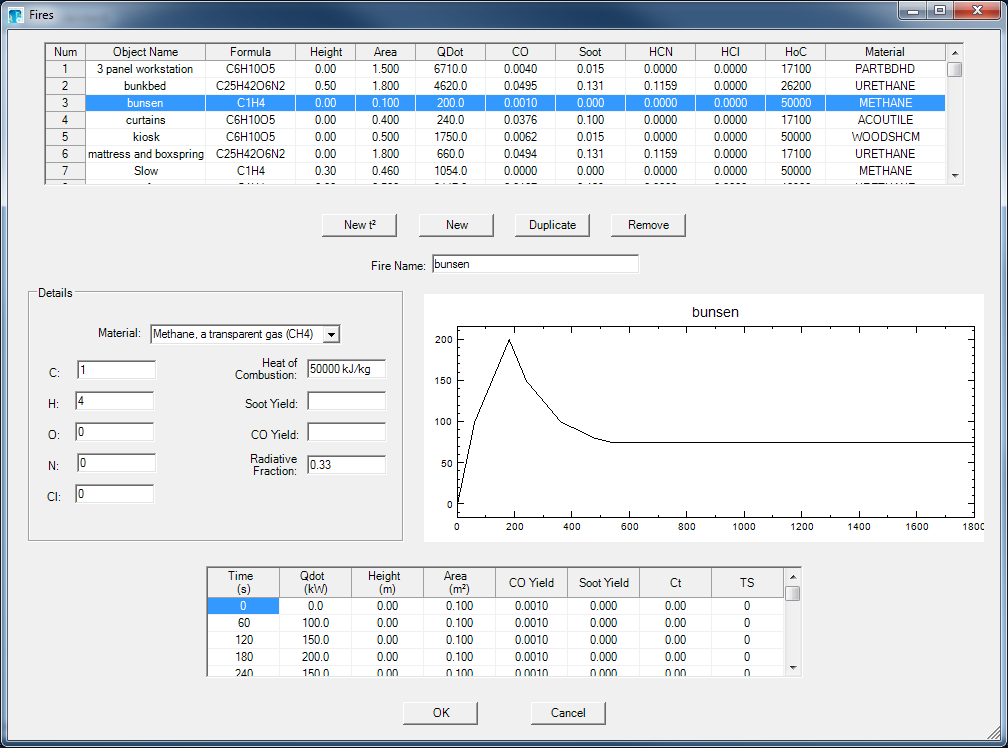
\includegraphics[width=6.5in]{FIGURES/Input_File/Fire_Object_Edit}
\end{center}
\end{figure}

\textbf{Fire Name:} The name from the collection of fire objects for the desired object.  This corresponds to the name of the fire object file, without the extension. Specifying a name not found in the database causes CFAST to stop with an appropriate error message.

\textbf{Material} (default value: none): material name from the thermal properties data file used for the object. The material properties are used to calculate heat transfer into the object from its surroundings.

\textbf{C, H, O, N, Cl}: Molecular formula of the burning fuel. Burning fuels in CFAST are assumed to be hydrocarbon fuels that contain at least Carbon and Hydrogen and optionally Oxygen, Nitrogen, and Chlorine. These five inputs define the stoiciometry of the fuel as it is burned.  Thus, for example, all of the specified Nitrogen and Chlorine is assumed to completely react to form HCN and HCl.  If only partial conversion is desired, a smaller ratio for Nitrogen and/or Chlorine can be specified.

\textbf{Heat of Combustion} (default units: J/kg, default value: 50 000 000 J/kg): The energy released per kilogram of mass burned.

\textbf{Soot Yield} (default units: kg/kg, default value: 0 kg/kg): Constant species yields of soot expressed as ratios of carbon to fuel produced by the pyrolysis of the fuel. This input allows the user to specify a single value for soot yield for all time points in the fire time line. Individual time points can be changed as desired in the spreadsheet input described below.

\textbf{CO Yield} (default units: kg/kg, default value: determined by correlation): Constant species yield of carbon monoxide expressed as a fraction of the fuel mass converted into carbon monoxide.  By default, the CO yield is related to the soot yield via the correlation developed by K\"oyl\"u and Faeth

\be
y_{CO} = \frac{12n_C}{M_fv_f}0.0014 + 0.37y_s \label{eq:Koylu} \ee
where $n_C$ is the number of carbon atoms in a fuel molecule, $M_f$ is the molecular weight of the fuel, and $v_f$ is the stoichiometric coefficient of the fuel, assumed to be 1 here \cite{Koylu:1991}. Note that this correlation refers to well-ventilated fires. Yields of CO and soot in underventilated fires is still a subject of active research.

\textbf{Radiative Fraction}: The fraction of the energy produced in combustion that is radiated from the fire and plume. Within CFAST, the radiative fraction defaults to 0.30 ; i.e., 30 \% of the fire’s energy is released via radiation.  For other fuels, the work of Tewarson \cite{Tewarson:2003}, McCaffrey \cite{McCaffrey:1982}, or Koseki \cite{Koseki:1989} is available for reference.  The typical range for the radiative fraction is from about 0.05 to 0.4.

\subsection{T-squared Fires}

For a wide range of fires, the fire growth can be accurately represented with a power law relation of the form $\dQ=\alpha t^2$  where $\dQ$  is the heat release rate of the fire, $\alpha$ is the fire intensity coefficient, and $t$ is time \cite{Schifiliti:2002}.

\begin{figure}[h!]
\begin{center}
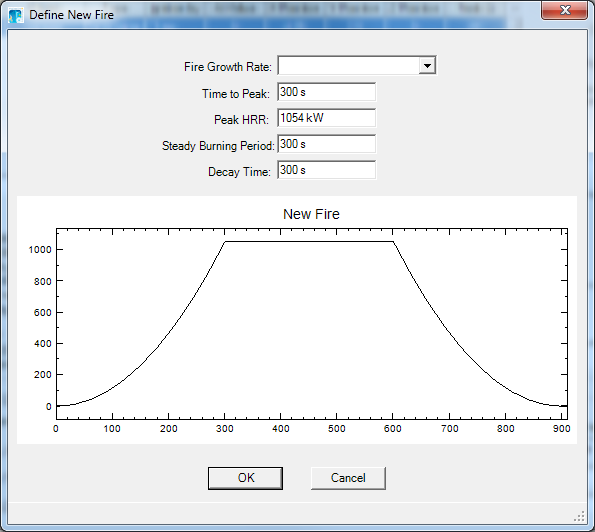
\includegraphics[width=5in]{FIGURES/Input_File/Create_t2}
\end{center}
\end{figure}

\textbf{Fire Growth Rate}: A set of specific t-squared fires labeled slow, medium, fast, or ultra-fast with fire intensity coefficients ($\alpha$) such that the fires reached 1054 kW (1000 BTU/s) in 600 s, 300 s, and 150 s, are available.  Each of these growth rates (with corresponding decay rates) can be selected. A fifth, custom, selection allows the user to define any growth or decay rate desired.

\textbf{Time to Peak}: (default units: s, default value: 300 s): The time for the fire to reach the peak fire size.

\textbf{Peak HRR}: (default units: kW, default value: 1054 kW): The peak heat release rate of the t-squared fire.  Fire size is constant beginning at a time consistent with the time to reach the peak value,   and continues at that value for the time specified in the steady burning period, below.

\textbf{Steady Burning Period}: (default units: s, default value: 300 s): Duration of time that the fire continues burning at the rate specified by the maximum HRR input, above.

\textbf{Decay Period}: (default units: s, default value, 300 s): Duration of time for the fire to decay back to a zero value.  Decay follows the inverse of the t-squared growth rate.

\begin{figure}[h!]
\begin{center}
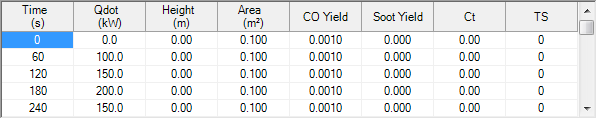
\includegraphics[width=6.219in]{FIGURES/Input_File/Fire_Spreadsheet}
\end{center}
\end{figure}

For all fires, including t-squared fires, values are calculated for time dependent variables, including default values for species generation. For all inputs, these values can be changed. All of the time dependent variables depend on a predefined time line. The time input specifies a sequence of time points that define the timing of the fire.  An entry indicates a point on the time-line when the mass loss rate, fuel height and other time dependent values are specified for the fire.  This time is independent of the simulation time which is specified by the TIMES line. If the simulation time is longer than the total duration of the fire, the final values specified for the fire (mass loss rate, fuel height, fuel area, and species) are continued until the end of the simulation.

\textbf{Time} (default units: s, default values: none): specify a sequence of time points that define the timing of the main fire.  An entry indicates a point on the time-line when the heat release loss rate, fuel height and other time dependent values are specified for the fire.

\textbf{Heat Release Rate (Qdot)} (default units: kW, default values: none): Heat release rate of the fire as a series of time points consistent with the time specification.

\textbf{Fire Height} (default units: m, default values: 0 m): Time-based values for height of the base of the fire.  Actual height of the base of the fire is the sum of the constant value specified for the fire and this height specification for a particular time in the fire development.

\textbf{Area} of the Base of the Fire (default units: m$^2$, default values: 0.3 m$^2$): Cross-sectional area of the base of the fire.

\textbf{CO Yield} (default units: kg/kg, default values: constant value from correlation, in eq. \ref{eq:Koylu}): yield of carbon monoxide expressed as a fraction of the fuel mass converted into carbon monoxide.

\textbf{Soot Yield} (default units kg/kg, default values: none): yield of soot expressed as a fraction of fuel mass converted into smoke paertiulate..

\textbf{Ct} (default units: kg/kg, default values: none): Yield of a fictitious toxic species per mass of fuel produced in the pyrolysis of the fuel. 

\textbf{TS} (default units: kg/kg, default values: none): Yield of user-defined trace species per mass of fuel produced in the pyrolysis of the fuel. 

\begin{itemize}
\item With the two parameters, heat of combustion ($H_C$) and heat release rate $\dQ$, the pyrolysis rate of the fuel is determined by $\dm=\frac{\dQ}{H_C}$.  
\item By default, the fire is placed in the center of the compartment on the floor.  If values for any of the three variables are invalid (i.e., less than zero or greater than the compartment dimension in the appropriate direction), the location for that direction defaults to the center of the appropriate direction. 
\item The area of the base of the fire should not be left at a value of zero. Radiation from the fire is determined by a point source calculation from the vertical center of the flame which is in turned determined by Heskestad's flame height correlation \cite{Heskestad:2002}, a function of heat release rate and fire area.
\item For “normally toxic” materials, Ct takes a value of 1 and is typically changed by an order of magnitude for particularly toxic or non-toxic materials.  It is not part of the mass balance for the fuel and system, but it just carried along as a transported species in flow through the structure. Ct is used as a measure of toxicity of a material.  Typically the integrated Ct versus time product is calculated. For normal materials, a concentration-time product of 900 mg min/m$^3$ is an indication of incapacitation.
\item The trace species is transported along with fire gases, but is assumed not to take part in the combustion reaction and is assumed not to be a significant source of overall mass for the system mass balance calculated by the model. This implies that the production rate of trace species specified should be much smaller than the total specified pyrolysis rate. If necessary, the trace species can be scaled to a smaller value (e.g., divided by 1000) for the simulation and converted back for analysis (e.g., multiplied by 1000).
\item In the input editor, time-dependent data are entered in a simple spreadsheet. Normal windows copy (Ctrl-C), cut (Ctrl-X), and paste (Ctrl-V) keyboard shortcuts are available for data editing. In addition, Alt-Ins will insert a complete row above the currently-selected row in the spreadsheet and Alt-Del will delete the current row in the spreadsheet.
\end{itemize}

\subsection{Associating Fire Objects with One or More Instances of the Fire in the Compartments of the Simulation}

Fires  are placed in defined positions within a compartment of a simulation and oriented with a normal vector to the surface of the object.  Ignition of an object may be at a specified time, a specified net incident heat flux on the surface of the object, or at a specified surface temperature of the object. The relevant CFAST keywords are FIRE, CHEMI, TIME, HRR, SOOT, CO, TRACE, AREA, and HEIGH.

\begin{lstlisting}
!!Wood_Wall
FIRE,1,4.55,2.5,0,1,1,0,0,0,1,Wood_Wall
CHEMI,1,4,0,0,0,0.33,1.81E+07,HARDWOOD
TIME,0,8000
HRR,0,1000000
SOOT,0.02,0.02
CO,0.02,0.02
TRACE,0,0
AREA,0.05,9
HEIGH,0,3
\end{lstlisting}

\begin{figure}[h!]
\begin{center}
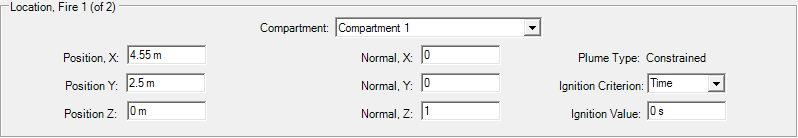
\includegraphics[width=6.5in]{FIGURES/Input_File/Fire_Positioning}
\end{center}
\end{figure}

\textbf{Compartment} of Fire Origin: specifies the compartment that contains the main fire for the simulation.  Any compartment defined is valid.

\textbf{Position X}: (default units: m, default value: compartment width / 2): Position of the center of the base of the fire measured in the x direction from the front lower left corner of the compartment origin (0,0,0) in the compartment of fire origin.

\textbf{Position Y}: (default units: m, default value: compartment depth / 2): Position of the center of the base of the fire measured in the y direction from the front lower left corner of the compartment origin (0,0,0) in the compartment of fire origin.

\textbf{Position Z}: (default units: m, default value: 0 m): Position of the center of the base of the fire measured in the z direction from the front lower left corner of the compartment origin (0,0,0) in the compartment of fire origin. Actual height of the base of the fire is the sum of the value specified by FPOS and by FHIGH for a particular time in the fire development.

\textbf{Normal  X} Component: specifies a vector of unit length perpendicular to the exposed surface of the object. (Depth) component is in the direction from the rear wall of the object compartment. Default value is a horizontal, upward facing object, unit vector = (0,0,1)

\textbf{Normal  Y} Component: specifies a vector of unit length perpendicular to the exposed surface of the object. (Breadth) component is in the direction from the left wall of the object compartment. Default value is a horizontal, upward facing object, unit vector = (0,0,1)

\textbf{Normal  Z} Component: specifies a vector of unit length perpendicular to the exposed surface of the object. (Breadth) component is in the direction from the floor of the object compartment. Default value is a horizontal, upward facing object, unit vector = (0,0,1)

\textbf{Plume Correlation}: specifies the algorithm used to calculate entrainment of air into the plume.  At present, a plume based on the work of McCaffrey or the work of Heskestad is allowed. By default, the McCaffrey plume is used.

\textbf{Ignition Criterion}: The type of ignition condition specified by the Ignition Criterion Value. Acceptable values are 1 for time, 2 for object surface temperature, and 3 for incident flux to object surface.

\textbf{Ignition Value}: The numerical value at which ignition will occur. If it is less than or equal to zero, the default value of zero is taken.

\subsection{Calculating Normal Vectors}

The general equations for determining the normal vectors in the x, y, and z directions are \\~

Normal vector in the x direction, $x = \sfrac{x}{\sqrt{x^2 + y^2 + z^2}}$ \\

Normal vector in the y direction, $y = \sfrac{y}{\sqrt{x^2 + y^2 + z^2}}$ \\

Normal vector in the z direction, $z = \sfrac{z}{\sqrt{x^2 + y^2 + z^2}}$ \\

The simplest way to calculate the unit vector is to draw an imaginary line at right angles (i.e., 90$^\circ$ angle) from the exposed surface of the target and to extend this imaginary line until it hits the walls, floor or ceiling of the compartment in which it is located.  This imaginary line is actually a vector that starts at the surface of the exposed target and terminates on a wall, floor, or ceiling.  Once the start point and the end point of a vector are known, the unit vector for this imaginary line may be calculated as follows:

\begin{equation}
  \begin{aligned}
 x &= \sfrac{x_{end} - x_{start}}{\sqrt{\brackets{x_{end} - x_{start}}^2 + \brackets{y_{end} - y_{start}}^2 + {z_{end} - z_{start}}^2}} \\
 y &= \sfrac{y_{end} - y_{start}}{\sqrt{\brackets{x_{end} - x_{start}}^2 + \brackets{y_{end} - y_{start}}^2 + {z_{end} - z_{start}}^2}} \\
 z &= \sfrac{z_{end} - z_{start}}{\sqrt{\brackets{x_{end} - x_{start}}^2 + \brackets{y_{end} - y_{start}}^2 + {z_{end} - z_{start}}^2}}
  \end{aligned}
\end{equation}

As an example, assume the following scenario:

\begin{itemize}
\item A square shaped target object is located in the middle of the floor of a compartment.
\item The target is constructed from no-combustible materials except the top.
\item The square shaped material is 1 m in depth, 1 m in breadth, and 1 m high.
\item The reference point (0,0,0) in the compartment is the lower left hand side of the rear wall.
\item The compartment is 3 meters in the x direction (i.e., the distance from the rear wall to the front wall of the compartment), 4 meters in the y direction (i.e., the distance from the left wall to the right wall of the compartment), and 5 meters in the z direction (i.e., the distance from the floor to the ceiling of the compartment).
\end{itemize}

Since the only side of the target that is combustible is the top surface of the target object, an imaginary line is draw perpendicular (i.e., at a 90$^\circ$ angle) from the top surface of the target object and extended until it reaches the outer boundary of the compartment.  In this case, since the top of the target object is facing the ceiling, the imaginary line would run straight up to the ceiling, running parallel to the four walls of the compartment, and terminating at the ceiling at the point (1.5 m, 2 m, 5 m).  Since the vector starts at point (1.5-m, 2-m, 1-m) and terminates at (1.5-m, 2-m, 5-m), the unit vectors can be calculated as follows:


\begin{equation}
  \begin{aligned}
 x &= \sfrac{x_{end} - x_{start}}{\sqrt{\brackets{x_{end} - x_{start}}^2 + \brackets{y_{end} - y_{start}}^2 + {z_{end} - z_{start}}^2}} &= \sfrac{1.5 - 1.5}{\sqrt{\brackets{1.5 - 1.5}^2 + \brackets{2 - 2}^2 + {5 - 1}^2}} \\
 y &= \sfrac{y_{end} - y_{start}}{\sqrt{\brackets{x_{end} - x_{start}}^2 + \brackets{y_{end} - y_{start}}^2 + {z_{end} - z_{start}}^2}} &= \sfrac{2 - 2}{\sqrt{\brackets{1.5 - 1.5}^2 + \brackets{2 - 2}^2 + {5 - 1}^2}} \\
 z &= \sfrac{z_{end} - z_{start}}{\sqrt{\brackets{x_{end} - x_{start}}^2 + \brackets{y_{end} - y_{start}}^2 + {z_{end} - z_{start}}^2}}  &= \sfrac{5 - 1}{\sqrt{\brackets{1.5 - 1.5}^2 + \brackets{2 - 2}^2 + {5 - 1}^2}} \\
  \end{aligned}
\end{equation}

In this case, the unit vector in the +Z direction.

\newpage
\section{Special Features}

The following section describe some special features that are only required for more advanced simulations with CFAST.

\subsection{Additional Thermal Properties}

The default CFAST installation includes a set of thermal properties for common building materials taken from textbook references.  While these may be useful for a range of problems, the user can also define additional materials for use with a specific simulation.

\subsection{Sprinklers and Detectors}

Sprinklers and detectors are both considered detection devices by the CFAST model and are handled using the same input keywords.  Detection is based upon heat transfer to the detector. Fire suppression by a user-specified water spray begins once the associated detection device is activated.  A maximum of 10 sprinklers or detectors can be included in a single compartment in a CFAST input file and model run. The DETEC keyword is used for both detectors and sprinklers. The first three parameters are required. The next three have defaults. The last three must be specified if the input is a heat detector or sprinkler.

\begin{lstlisting}
!!
!!target and detector keywords
!!
DETECT,2,1,347.04,4.55,2.5,4.554,100,1,7E-05
\end{lstlisting}


\begin{figure}[h!]
\begin{center}
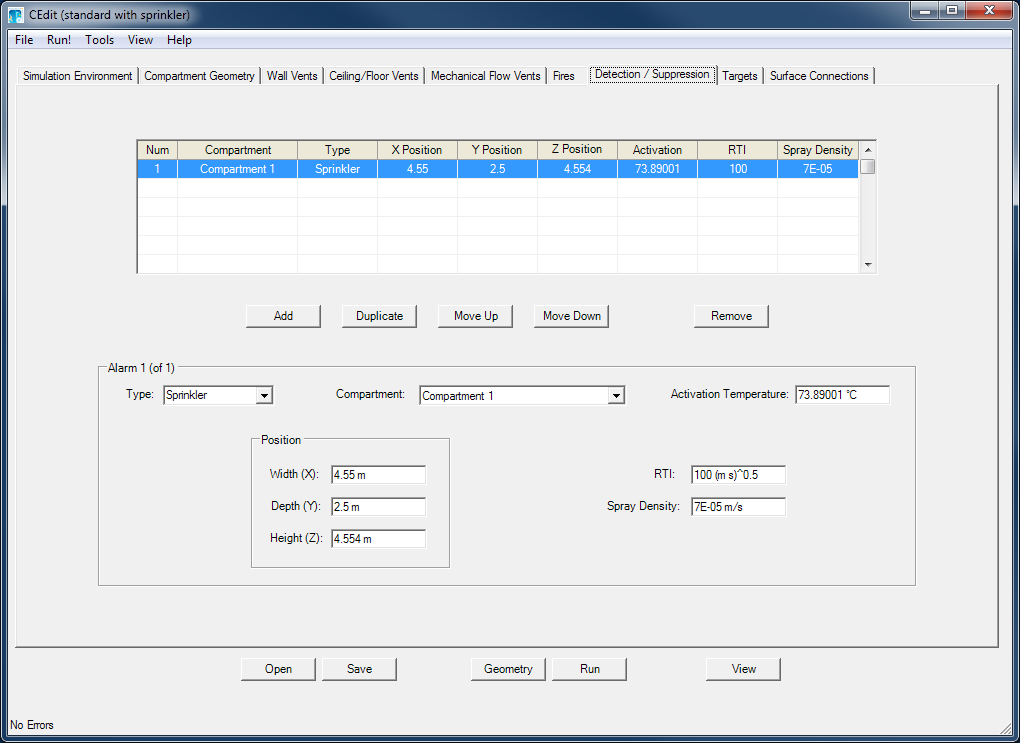
\includegraphics[width=6.5in]{FIGURES/Input_File/Detector_Tab}
\end{center}
\end{figure}

\textbf{Type}: type of detector, select smoke detector, heat detector, or sprinkler.

\textbf{Compartment}: the compartment in which the detector or sprinkler is located.

\textbf{Activation Temperature} (default units: \degc, default value: dependent on type): the temperature at or above which the detector link activates.

\textbf{Width (X}) Position (default units: m, default value: none): position of the object as a distance from the left wall of the compartment (X direction).

\textbf{Depth (Y}) Position (default units: m, default value: none): position of the detector or sprinkler as a distance from the front wall of the compartment (Y direction).

\textbf{Height (Z)} Position (default units: m, default value: none): position of the object as a distance from the floor of the compartment (Z direction).

\textbf{RTI} (default units: (m ∙ s)1/2, default value: none): the Response Time Index (RTI) for the sprinkler or detection device.

\textbf{Spray Density} (default units: m/s, default value: none): the amount of water dispersed by a water spray-sprinkler.  The units for spray density are length/time.  These units are derived by dividing the volumetric rate of water flow by the area protected by the water spray. The suppression calculation is based upon an experimental correlation by Evans , and depends upon the RTI, activation temperature, and spray density to determine the behavior of the sprinkler.

\begin{itemize}
\item Often, the activation of smoke alarms is simulated with a temperature-based criterion, typically in the range of 5~\degc to 10~\degc above ambient. Davis and Notarianni  studied the activation of heat and smoke alarms in small and large compartments \cite{Davis:1996}. They conclude that a temperature rise of approximately 5~\degc corresponded to activation of ionization alarms for a range of fire sources and ceiling heights. The Nuclear Regulatory Commission includes a default value of 10~\degc in NUREG-1805 \cite{NRCNUREG1805} .
\item Several cautions should be observed when using estimates of sprinkler suppression within the model: 1) the first sprinkler activated controls the effect of the sprinkler on the heat release rate of the fire.  Subsequent sprinklers which may activate have no additional effect on the fire simulation. 2) The fire suppression algorithm assumes the effect of the sprinkler is solely to reduce the heat release rate of the fire. Any effects of the sprinkler spray on gas temperatures or mixing within the compartment are ignored. 3) The sprinkler always reduces the heat release rate of the fire. The ability of a fire to overwhelm an under-designed sprinkler is not modeled. 4) Since the dynamics of the sprinkler and direct effects of the spray on gas temperatures and velocities are not modeled, calculated times of activation of secondary sprinklers and / or detectors after the first sprinkler is activated should be not be modeled since the impact of the first sprinkler on the activation of additional sprinklers is not included in the CFAST model.
\end{itemize}

\subsection{Defining Targets}

CFAST can track and report calculations of the net heat flux striking arbitrarily positioned and oriented targets and the temperature of these targets.  The relevant keyword used to specify targets is TARGE. 

\newpage

\begin{lstlisting}
!!
!!Target and detector keywords
!!
TARGET,1,2.2,1.88,2.34,0,0,1,CONCRETE,IMPLICIT,PDE,0.5
\end{lstlisting}

In addition to any user-defined targets, there are always two targets that are automatically placed in any compartment containing a fire. Both are included for reporting purposes. The first is an “ambient target” and is intended to represent the net flux to a human body. This is used for the flux in the hazard calculation for tenability. The assumption is that the target will remain at ambient temperature, which is a surrogate for body temperature. The second determines the net flux to a horizontal target on the floor whose temperature is assumed to be the same as the floor surface. The calculation can be used to estimate the ignition of combustibles on the floor as a surrogate for estimating time to flashover, typically taken to be 20 kW/m$^2$. Thus if one of the target keywords is used, it will be in addition to these two predefined targets.

\begin{figure}[h!]
\begin{center}
\includegraphics[width=6.5in]{FIGURES/Input_File/Target_Tab}
\end{center}
\end{figure}

For all targets, heat flux is calculated to the surface specified by the user (with the direction determined by the normal vector). Conduction into the target is assumed to occur only from this surface into the target.


\textbf{Compartment}: The compartment in which the target is located.

\textbf{Width (X)} Position (default units: m, default value: none): Position of the target as a distance from the left wall of the target compartment (X direction).

\textbf{Depth (Y)} Position(default units: m, default value: none): Position of the target as a distance from the front wall of the target compartment (Y direction).

\textbf{Height (Z)} Position(default units: m, default value: none): Height of the target above the floor (Z direction).

\begin{wrapfigure}{r}{0pt}
  \includegraphics[width=1.875in]{FIGURES/Input_File/Target_Points_To}
\end{wrapfigure}

\textbf{Normal Vector X} Component: specifies a vector of unit length perpendicular to the exposed surface of the target. (Width) component in the direction from the left wall of the target compartment. A value of 1 defines a vertical target facing into the compartment, unit vector = (1,0,0). The X, Y, and Z component of the normal vector can also be calculated automatically with a pull down menu that allows selection of surfaces and fires in the compartment visible from the target location.

\textbf{Normal Vector Y} Component: specifies a vector of unit length perpendicular to the exposed surface of the target. (Depth) component in the direction from the front wall of the target compartment. A value of 1 defines a vertical target facing to the right, unit vector = (0,1,0). 

\textbf{Normal Vector Z} Component: specifies a vector of unit length perpendicular to the exposed surface of the target. (Height) component in the direction from the floor of the target compartment. Default value is a horizontal, upward facing target, unit vector = (0,0,1).

\textbf{Material}: Used to specify the wall material of the target.  Any material from the thermal database used to represent wall materials may be used here.  Since the transient heat conduction problem is not solved now for the target this parameter is not used. 

\textbf{Target Type}: If the solution method is not STEADY, this parameter further indicates the solutions equations.  Specifiy Thermally Thick, Thermally Thin, or Cylindrical.  For thermally thin materials, CFAST uses ordinary differential equations; for thermally thick materials, partial differential equations, and for cylindrical targets, cylindrical corrdinates.

\textbf{Solution Method}: Optional parameter that indicates the solution method. STEADY for steady state solution, EXPLICIT for explicit solution, IMPLICIT for implicit solution.

\begin{itemize}
\item The TARGE keyword performs a heat transfer calculation between the compartment and the target. The steady state option assumes that the target material reacts instantly to changing conditions and computes the target temperature that would result in a balance of incoming and outgoing heat (i.e., a steady state). If a transient target temperature is modeled, then one can either assume that there is a temperature variation within the target or assume that the target is “thin” and can be modeled using only one temperature. If the target is assumed to be thin then the ODE option should be used set since this is how the equations are solved. If the target is assumed to be thick then the PDE option should set. Finally, if one of the two transient options are set (ODE or PDE), the numerical solution can be solved using an explicit or an implicit method.  Typically, the implicit method will work in all cases.  The explicit method is recommended only when the implicit method fails to come to a solution.

\end{itemize}

\subsection{Modeling a Compartment as a Tall Shaft or Long Corridor}

For tall compartments or those removed from the room of fire origin, the compartment may be modeled as a single, well-mixed zone rather than the default two-zone assumption. A single zone approximation is appropriate for smoke flow far from a fire source, where the two-zone layer stratification is less pronounced than in compartments near the fire. This is used in situations where the stratification does not occur. Examples are elevators, shafts, complex stairwells, and compartments far from the fire.

For long hallways or corridors, there can be a significant delay time for the initial hot gas layer to travel along the ceiling to the far end of the compartment. By estimating the time required for a ceiling jet to travel in a corridor and the temperature distribution along the corridor, CFAST can delay flow into compartments connected to corridors until the ceiling jet has passed the connections to these compartments.

\begin{figure}[h!]
\begin{center}
\includegraphics[width=4.5in]{FIGURES/Input_File/Corridor_Flow}
\end{center}
\end{figure}

\textbf{50 \% Decay Velocity} (default units: m/s, default value: calculated by software): ceiling jet velocity at the distance from the reference point where the temperature falls off by 50 \%. Default velocity and depth are calculated by the program based on the vent size, flow and layer thickness in the horizontal vent from which flow first enters the hallway, and on the width of the hallway1.

\textbf{50 \% Decay Depth} (default units: m, default value: calculated by software): ceiling jet depth at the distance from the reference point where the temperature falls off by 50 \%. 

\textbf{50 \% Decay Distance} (default units: m, default value: calculated by software): distance from the reference point where the temperature falls off by 50 \%.

\begin{itemize}
\item  Since the algorithm depends on the flow into the hallway to determine default ceiling jet velocity and depth, the main fire compartment should not be specified as a hallway. In the main fire compartment, a stable layer will build before flow into the compartment through horizontal vents.
\item The zone model concept best applies for an enclosure in which the width and length are not too different.  If the horizontal dimensions of the room differ too much (i.e., the room looks like a corridor), the flow pattern in the room may become asymmetrical. If the enclosure is too shallow, the temperature may have significant radial differences. The width of the plume may at some height become equal to the width of the room and the model assumptions may fail in a tall and narrow enclosure. Therefore, the user should recognize approximate limits on the ratio of the length (L), width (W), and height (H) of the compartment. 
\item If the aspect ratio (the maximum of length/width or width/length) is greater than about 5, the corridor flow algorithm can be used to provide the appropriate filling time. By contrast, a single zone approximation is more appropriate for tall shafts (elevators and stairways).  This is due to interaction of the plume, lower layer, and shaft walls that leads to complete mixing.  This is the inverse of the corridor problem, and occurs at an aspect ratio (the maximum of height/width or height/length) of about 5. Recommended guidance is as follows:  If the width to length aspect ratio (the maximum of length/width or width/length) is greater than 5, use of the corridor flow algorithm is appropriate. If the width to length aspect ratio is greater than 3 but less than 5, the corridor flow algorithm may or may not be appropriate; consider the results from a simulation with and without the algorithm to assess its appropriateness. If the room is not a corridor and the height aspect ratio (the maximum height/width or height/length) is greater than 5, the single zone approximation is appropriate.
\end{itemize}

\subsection{Defining Compartment Area}

The Compartment Geometry page includes two additional entries that may be used for defining compartment properties for spaces which are not rectangular in area.  Values are entered in a spreadsheet. The CFAST keywords ROOMA and ROOMH keywords allow the user to define non-rectangular rooms by specifying cross-sectional area as a function of height. One set of values is included for each compartment that has a variable cross-sectional area.

\begin{lstlisting}
!!
!!Compartment keywords
!!
ROOMA,1,6,700.04,700.04,571.44,571.44,411.44,411.44
ROOMH,1,6,0,1.799,1.8,2.199,2.2,2.399
\end{lstlisting}

\begin{figure}[h!]
\begin{center}
\includegraphics[width=4.5in]{FIGURES/Input_File/Variable_Area}
\end{center}
\end{figure}
 
\textbf{Height Value(s)} (default units: m, default values: none): Values of height for the corresponding cross-sectional area values measured from the floor of the compartment. The values for the compartment correspond to cross-sectional area values included for the same compartment on the ROOMA command.

\textbf{Area Value(s)} (default units m$^2$, default values: none): Values of cross-sectional area of the compartment as a function of height measured from the floor of the compartment. The values for the compartment correspond to height values included for the same compartment on the ROOMH command.

\subsection{Surface Connections}

The Surface Connections page allows the user to define heat transfer between compartments in a simulation. Energy can be transferred from compartment to compartment through solid boundaries (walls, ceilings and floors) by means of conduction. The heat transfer between connected compartments is modeled by merging the connected surfaces for the ceiling and floor compartments or for the connected horizontal compartments.  The heat conduction problem is solved for the merged walls using a temperature boundary condition for both the near and far wall. As before, temperatures are determined by the solver so that the heat flux striking the wall surface (both interior and exterior) is consistent with the temperature gradient at that surface.  This option is implemented with the VHEAT (for vertical heat transfer) and the HHEAT (for horizontal heat transfer) keywords. 

\begin{figure}[h!]
\begin{center}
\includegraphics[width=6.5in]{FIGURES/Input_File/Surface_Connection_Tab}
\end{center}
\end{figure}

\textbf{Vertical Connections}: Heat transfer by conduction  between the ceiling and floor of specified compartments is included with the VHEAT keyword. Ceiling to floor heat transfer occurs between interior compartments of the structure or between an interior compartment and the outdoors. The model checks to make sure that the ceiling and floor are reasonably contiguous (within 0.01 m).  The assumption is made that this is true for the entire ceiling and floor. \\~ \\

\begin{lstlisting}
!!
!!Heat flow keywords
!!
VHEAT,2,1
\end{lstlisting}

\textbf{Horizontal Connections}: Heat transfer byl conduction between specified compartment wall surfaces is included with the HHEAT keyword.  Conduction through vertical partitions (walls) occurs between interior compartments of the structure or between an interior compartment and the outdoors.

\begin{lstlisting}
!!
!!Heat flow keywords
!!
HHEAT,2,1
\end{lstlisting}
 
\textbf{First Compartment}: First of the connected compartments. Order of the inputs is not important.

\textbf{Second Compartment}: Second of the connected compartments. Order of the inputs is not important.

\textbf{Fraction}: Specifies the fraction of the vertical surface areas of the compartments which are connected can be specified. The fraction specifies the fraction of the vertical surface area connecting the first and second compartment pair.

\textbf{Top Compartment}: The top or first of the two compartments to be connected by a vertical heat transfer connection. The connection is through the floor of this compartment.

\textbf{Bottom Compartment}: The bottom or second of the two compartments to be connected by a vertical heat transfer connection. The connection is through the ceiling of this compartment.

\subsection{The Ceiling Jet – An Additional Zone}

Typically, zone models incorporate two zones in each compartment, one for the upper layer and one for the lower layer. A plume from a fire then pumps energy from the fire and lower layer into the upper layer. However, it has been observed that the heat loss from the upper layer to the ceiling and walls is higher than this paradigm would indicate. The cause is that a plume does not initially mix with the upper layer. This leads to higher convective heat transfer than the mixed model would indicate. CFAST has incorporated a model of this additional heat loss based on the work of Cooper \cite{Cooper:1988} . Heat loss by this mechanism to the ceiling is well established, the loss to walls is somewhat more uncertain due to the uncertainty of how far the plume descends below the ceiling. 

\begin{wrapfigure}{r}{0pt}
  \includegraphics[width=2.313in]{FIGURES/Input_File/Ceiling_Jet}
\end{wrapfigure}

To include ceiling jet effects in the calculation of the surface temperature of the ceiling, wall, or both surfaces, the CJET keyword is used.  In the input editor, CEdit, this is included on the fires tab. The ceiling jet calculation can be used for the ceiling, walls, or all surfaces. At present, this keyword effects only the calculation of the convective heating boundary condition for the conduction routines.  If a particular surface is on, the ceiling jet algorithm is used to determine the convective heating of the surface.  If the ceiling jet is off, the bulk temperature of the upper layer determines the convective heating.

\begin{itemize}
\item Using this option affects all fires.”
\end{itemize}

\subsection{Filtering}
 
For mechanical vents, there are two species that can be filtered out of the gas flow: soot and the user-defined trace species. Filters are applied only to fan openings. The fan must have been defined before the filter can be applied. Initially filtering is off. It is turned on with the EVENT key word, defined in the input editor with a Filter Efficiency and Begin Filter At time. The relevant CFAST keyword is EVENT.

\begin{figure}[h!]
\begin{center}
\includegraphics[width=6.5in]{FIGURES/Input_File/Filtering}
\end{center}
\end{figure}

\textbf{Filter Efficiency} (default units:~\%, default value: none): Flow through mechanical vents may include filtering that removes a user-specified portion of soot and trace species mass from the flow through the vent.  By default, there is no filtering applied, that is all of the soot and trace species mass in the vent flow is passed through the vent. Within the user interface, this is specified as a filter efficiency of 0~\%.  If desired, the user may specify the fraction of the soot and trace species mass to be removed as a percentage.

\textbf{Begin Filtering At Time} (default units: s, default value: none): Time during the simulation at which the mechanical vent filtering begins.

\begin{itemize}
\item If the simulation includes mechanical ventilation filtering, care should be taken in choosing trace species production rates to insure the production rate is small compared to the total pyrolysis rate.  This will allow appropriate conservation of mass in the solution of the system of differential equation.  For large production rates of trace species, scaling factors can be used (e.g., divide by 1000) for the trace species production rate to reduce the relative magnitude compared to the pyrolysis rate.  For analysis, the resulting trace species in compartments and filters can be converted back to original units multiplying by the scaling factor used.
\end{itemize}